%------------------------------------------------------------------------------------------------------------------------%
\subsection{Complexity Analysis}\label{sect:alg_complexity}
%------------------------------------------------------------------------------------------------------------------------%
We now derive the computational complexity of using Algorithm~\cref{alg:refSeries} to solve an inference problem, and compare it to extant strategies. Let the state, adjoint, and parameter variables each have $N$ degrees of freedom, and assume that an `all at once' strategy is used to solve the KKT system. The cost of single linear solve with such a system is $\orderof{3N}^{\gamma}$, where $\gamma$ depends on the linear solver used~\cite{}. The cost of solving for the auxiliary variables, a linear system, is $\orderof{3N}^{\gamma}$. \red{The parts of the supplementary adjoint corresponding to the primary and auxiliary variables can be solved separately, and thus the cost of computing the supplementary adjoint is also $\orderof{3N}^{\gamma}$.}

If one utilizes Algorithm~\cref{alg:refSeries} to solve the inference problem, with $T$ adaptive iterations the total computational cost is,
%
\begin{align}
\label{eq:cost_adapt}
C_{MF} &= \sum_{i=1}^{T}L_{i}(3N)^{\gamma} + 1(3N)^{\gamma} + 2(3N)^{\gamma} \nonumber \\
&= \sum_{i=1}^{T} (L_i + 3) (3N)^{\gamma}
\end{align}
% 
where $L_i$ is the number of nonlinear solver steps needed to solve the KKT system for the low or mixed fidelity model at each adaptive step. The corresponding cost for solving the high fidelity inference problem, with a nonadaptive algorithm, based on a continuation scheme is,
%
\begin{equation}
\label{eq:cost_nadapt}
C_{HF} = \sum_{i=1}^{C}K_{i}(3N)^{\gamma}
\end{equation}
% 
where $K_i$ is the number of nonlinear solver steps needed to solve the KKT system for the high fidelity model at each continuation step, and $C$ is the number of continuation steps.

Comparing Eq.~\eqref{eq:cost_adapt} and~\eqref{eq:cost_nadapt}, we have,
%
\begin{equation}
\label{eq:cost_compare_0}
C_{MF} < C_{HF} \implies \sum_{i=1}^{T} (L_i + 3) < \sum\limits_{i=1}^{C}K_{i}
\end{equation}
%
If the low and multi-fidelity models are linear, or nonlinear in a very small region, then $L_i \approx 1$, and we have the following condition,
%
\begin{equation}
\label{eq:cost_compare_1}
T < \frac{\sum\limits_{i=1}^{C}K_{i}}{4},
\end{equation}
% 
for the adaptive algorithm to be less costly than solving the high-fidelity inverse problem. \red{I'm not sure this section makes sense, since this doesn't seem to hold for any of the actual runs we've done...our mixed models take fewer nonlinear steps than the HF model, but not close enough to one...}

%
%
%
%
%
%
%
%

\red{\Cref{alg:refSeries} can be naturally extended to an online-offline setting, where a multi-fidelity model adaptive constraint can be generated for a given data set in the offline phase. In the online phase, additional data points are added to the data set, and instead of solving the complete inverse problem with all the data points, and the high-fidelity constraints, an iterative algorithm can be initiated using the multi-fidelity representation developed in the offline phase. The adaptive procedure, with the supplementary adjoint can be used to adapt the preexisting multi-fidelity representation to the new data points. } 
%
\alglanguage{pseudocode}
\begin{algorithm}[h!]
\small
\caption{An algorithm to adapt a pre-computed mixed-fidelity model to new data.}
\label{alg:refonoff}
\begin{algorithmic}[1]
\State{Define maximum acceptable absolute relative QoI error \texttt{errTol}}
\State{Given a data set $d_1 \in \R^{n_{d_1}}$, and an adaptively build a mixed-fidelity model for low error in the QoI, use \cref{alg:refSeries} to build a MF model MF$_1$} 
\Procedure{$\texttt{Online}$}{HF model, MF model MF$_1$, \texttt{errTol}, $d_2 \in \R^{n_{d_2}}$}
	\State{$i\gets1$}
	\State{Solve for stationary point $\Psi_{MF_1}$ of augmented Lagrangian $\mathcal{M}_{MF_1}$ formed using new data set $d_2$}
	\State{Solve QoI error adjoint equation, linearized about $\Psi_{MF_1}$, for \par\hskip\algorithmicindent supplementary adjoint $\Lambda_1$ (see \cref{eq:superAdjEq})}
	\State{Compute QoI error estimate
		
	$\epsilon_0=-\frac{1}{2}\mathcal{M}'_{HF,\Psi}(\Psi_{MF_1})(\Lambda_1)+\mathcal M_{HF}(\Psi_{MF_1})-\mathcal M_{MF_1}(\Psi_{MF_1})$}
	\State{Calculate QoI $I(q_{MF_1},u_{MF_1})$}
	\While{$i<$ \texttt{maxIter} and $|\epsilon_i/I(q_{MF_i},u_{MF_i})|>$ \texttt{errTol}}
		\State{\begin{varwidth}[t]{\linewidth}Localize $\epsilon_i$ (see \cref{sec:errLocal}) and use this decomposition to guide \par\hskip\algorithmicindent formation of new mixed-fidelity model MF$_{i+1}$\end{varwidth}}
		\State{$i\gets i+1$}
		\State{Solve for stationary point $\Psi_{MF_i}$ of augmented Lagrangian $\mathcal{M}_{MF_i}$}
		\State{Solve QoI error adjoint equation, linearized about $\Psi_{MF_i}$, for 
		
		$\quad\quad$supplementary adjoint $\Lambda_i$ (see \cref{eq:superAdjEq})}
		\State{Compute QoI error estimate
		
		$\quad\quad \epsilon_i=-\frac{1}{2}\mathcal{M}'_{HF,\Psi}(\Psi_{MF_i})(\Lambda_i)+\mathcal M_{HF}(\Psi_{MF_i})-\mathcal M_{MF_i}(\Psi_{MF_i})$}
		\State{Calculate QoI $I(q_{MF_i},u_{MF_i})$}
	\EndWhile \\
\Return{QoI estimate $I(q_{MF_i},u_{MF_i})$ for the new data set $d_2$}
\EndProcedure
\Statex
\end{algorithmic}
\end{algorithm}
%
\Cref{alg:refonoff} lends itself to a quasi-incremental data assimilation approach, where the data set $d_2$ is an augmentation of the original set $d_1$. In such a situation, we expect that the model refinement will be concentrated around the new data points, that also inform the QoI. Thus, in the online phase, even though the inverse problem will be solved with all data points, the use of high-fidelity models will be limited, and the bulk of the computation (computing the auxilary variables, and supplementary adjoint) will be focused on identifying those new data points, which have the maximum impact on the QoI.

%
%
%
%
%
%
%
%
%
%

%------------------------------------------------------------------------------------------------------------------------%
\subsection{Constant vs Field Parameters} \label{sec:constvfield}
%------------------------------------------------------------------------------------------------------------------------%
It is not necessary for the low- and high-fidelity models to differ in the physics included. A low-fidelity model may be more computationally tractable due to a reduced number of degrees of freedom rather than reduced nonlinearity. In this section, we consider two models which differ in the space to which the parameter belongs, with the low-fidelity model having fewer degrees of freedom.
%------------------------------------------------------------%
\subsubsection{Problem Setup}
%------------------------------------------------------------%
We consider the same high-fidelity model as in \cref{sec:cdvcdr}:
\begin{equation}
k_d\nabla^2 u - \vec{V}\cdot\nabla u + k_ru^2= f(q),\quad q\in U,
\end{equation}
with the same diffusion coefficient $k_d = 0.1$  and reaction coefficient $k_r = -42$. The low-fidelity model
\begin{equation}
k_d\nabla^2 u - \vec{V}\cdot\nabla u + k_ru^2= f(q),\quad q\in\R
\end{equation}
differs from the high-fidelity model only in that the parameter $q$ is a constant instead of a field. Then the intermediate mixed-fidelity models have parameter fields which are non-constant in only portions of the domain. For ease of implementation, we require that the resulting parameter field remain continuous at the interface between the low-fidelity and high-fidelity subdomains, although this constraint is not necessary for the theory to hold. The domain, mesh, boundary conditions, and velocity field, as well as the observations, unknown parameters to be inferred, and QoI, remain the same as described in \cref{sec:cdvcdr}. As the inverse problem is ill-posed, except for perhaps in the case where the low-fidelity model is used throughout the domain, regularization is added; the Tikhonov regularization term is $\frac{\beta}{2}\int_\Omega \|\nabla f(q)\|_2^2+f(q)^2\:\textrm{d}A$, where $\beta=10^{-3}$ is a regularization coefficient.

Although using such a pair of models has similarities to the problem of adaptive mesh refinement, we note that in this example only the parameter field changes in its level of refinement, not the state. Should the two models differ in the resolution of the state variables instead of the parameters, it is more efficient to use the approach discussed in \cite{BecVex05}.
%------------------------------------------------------------%
\subsubsection{Adaptive Model Refinement Results}
%------------------------------------------------------------%
As with the previous examples in \cref{sec:cdvcdr}, the decomposition \cref{eq:basisblame} of the error estimate is used to select additional regions of the domain in which to use the high-fidelity model. The number of degrees of freedom in the inverse problem increases with the proportion of the domain in which the high-fidelity model is used and the unknown parameter allowed to be a field. With each iteration, an additional $10\%$ of the elements are marked for refinement. This is repeated until the estimated absolute relative error in the QoI, is less than $1\%$.

\Cref{fig:svfRef} shows the local error contributions, as well as the subdomains where the low- and high-fidelity models are used, for the first two and last mixed-fidelity model thus generated. Each linear Langrange basis function's contribution is plotted at its nonzero node. 
%
\begin{figure}[htbp]
\centering
\subfloat[MF$_0$ ($0\%$ HF)]{
	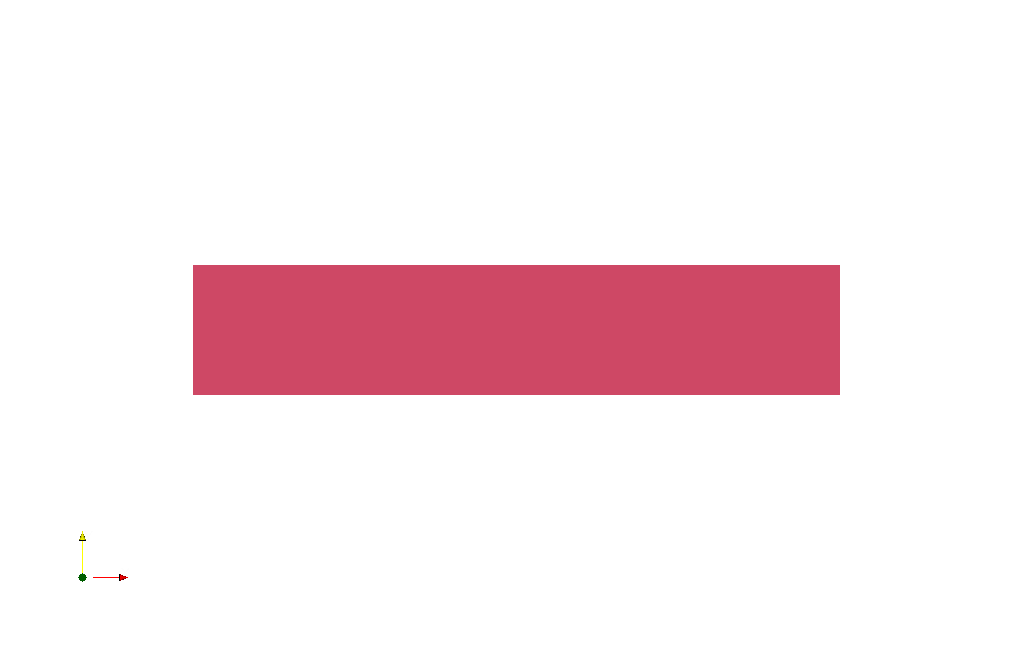
\includegraphics[width=0.46\textwidth]{svf/cd_cdr_LF_divvy.png}
  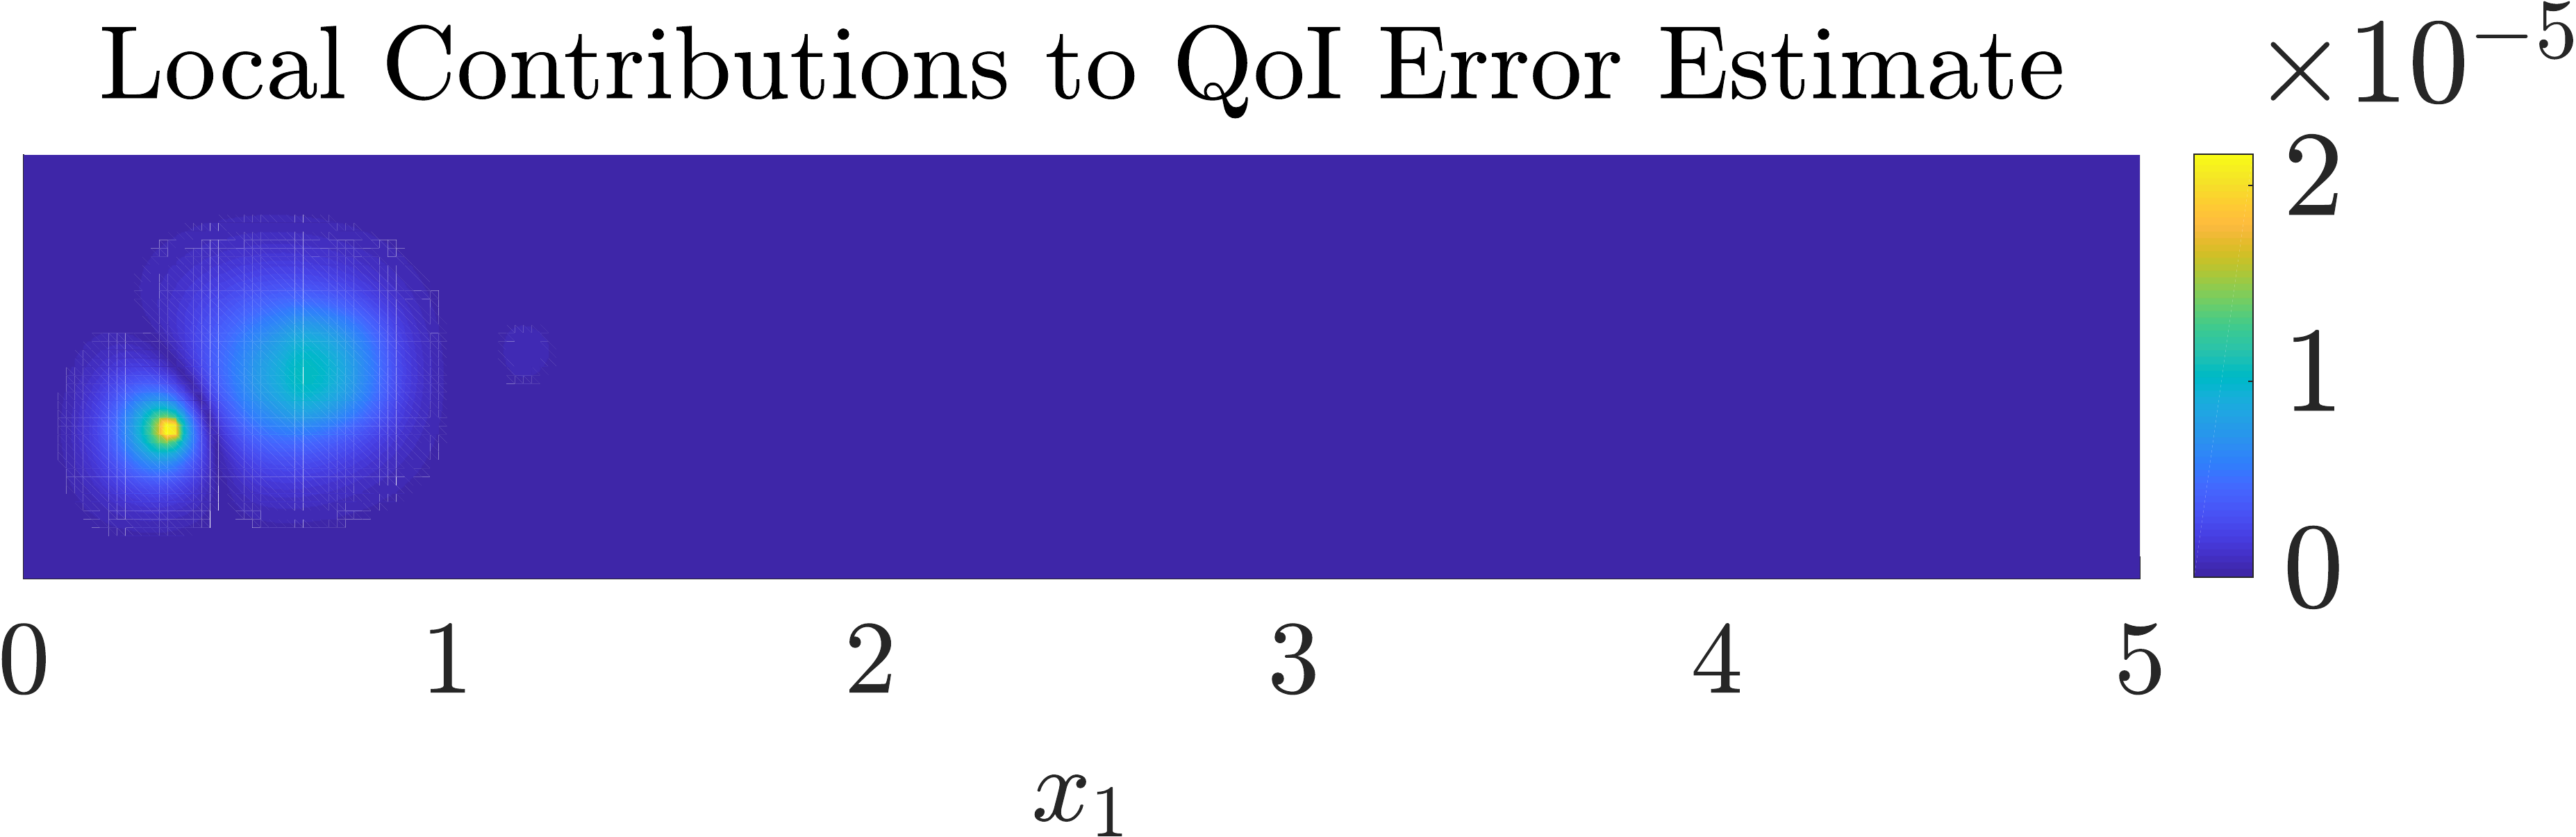
\includegraphics[width=0.49\textwidth]{svf/err_breakdown_LF.png}
} \\
\subfloat[MF$_1$ ($10\%$ HF)]{
	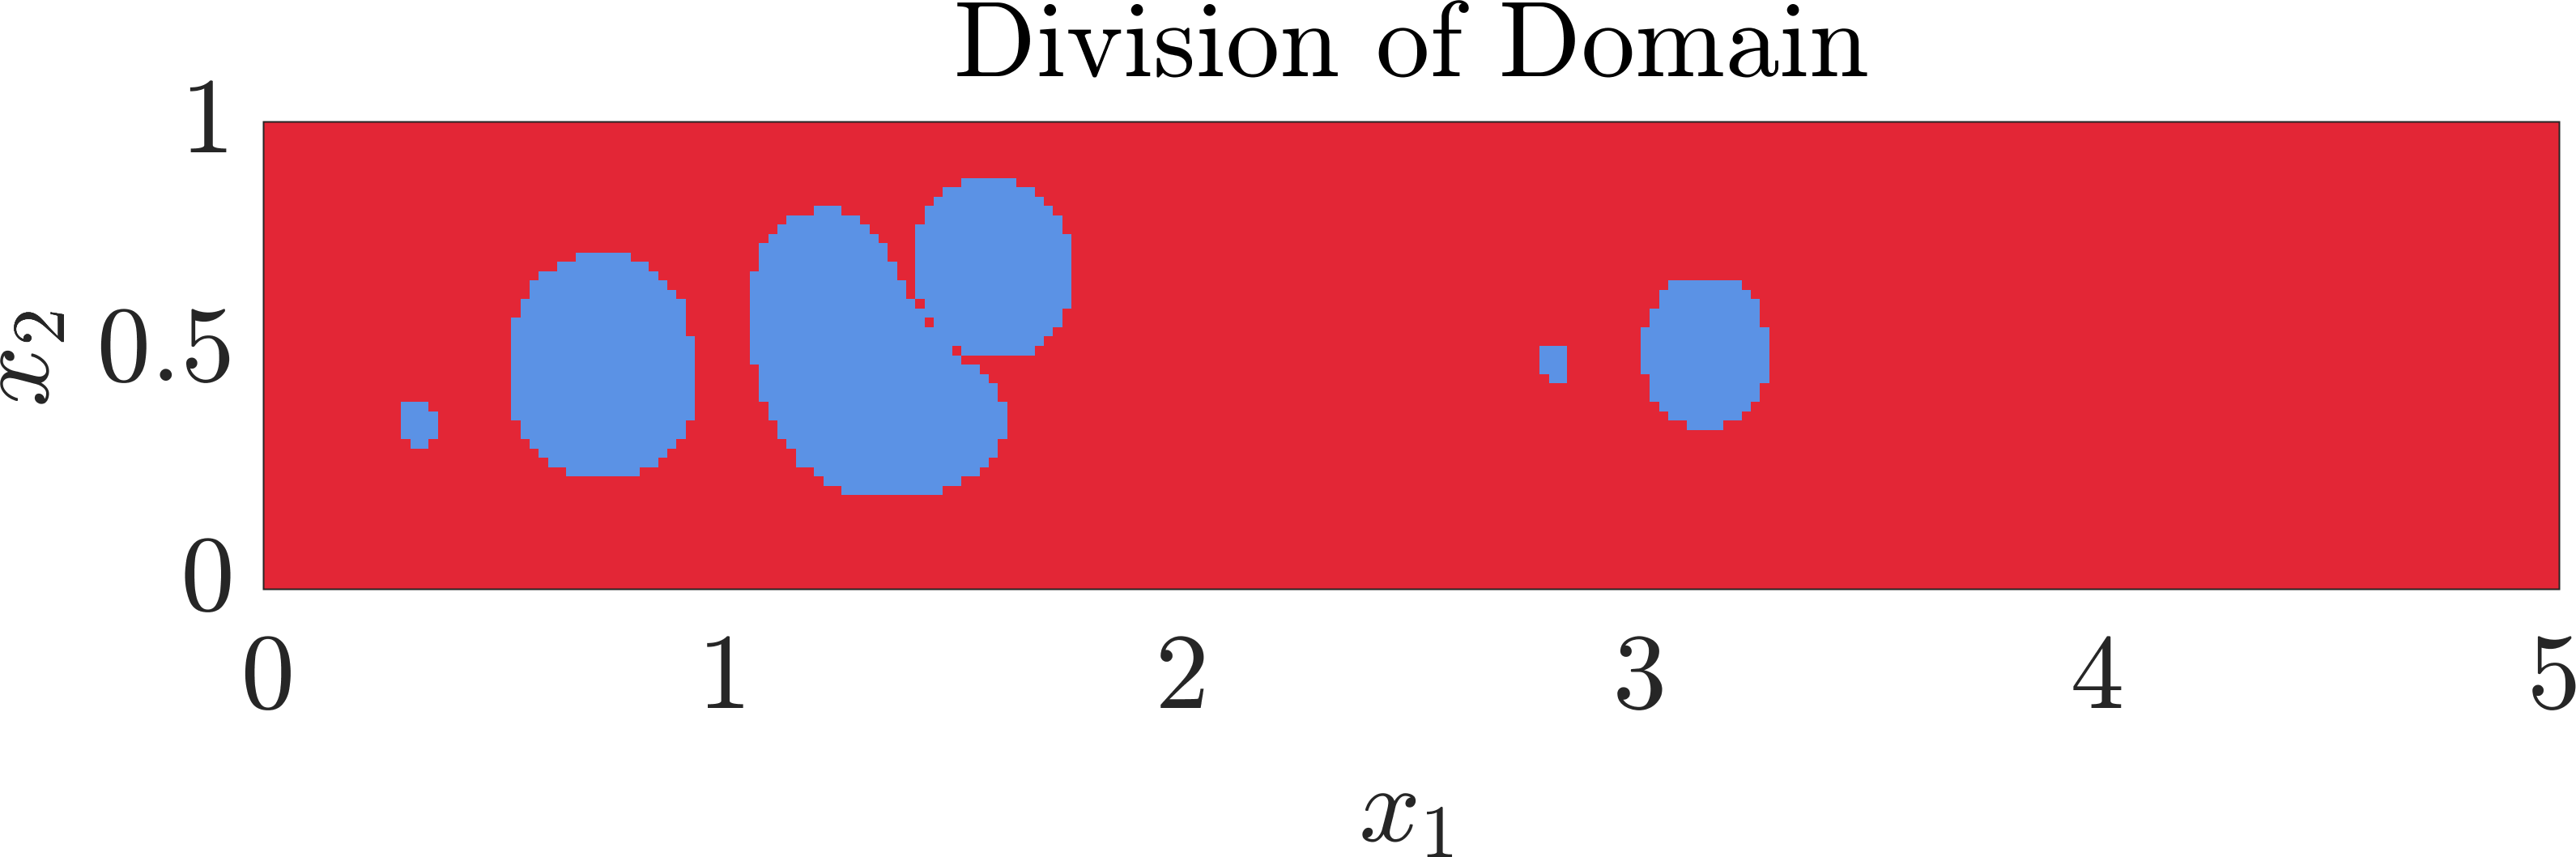
\includegraphics[width=0.46\textwidth]{svf/cd_cdr_MF01_divvy.png}
  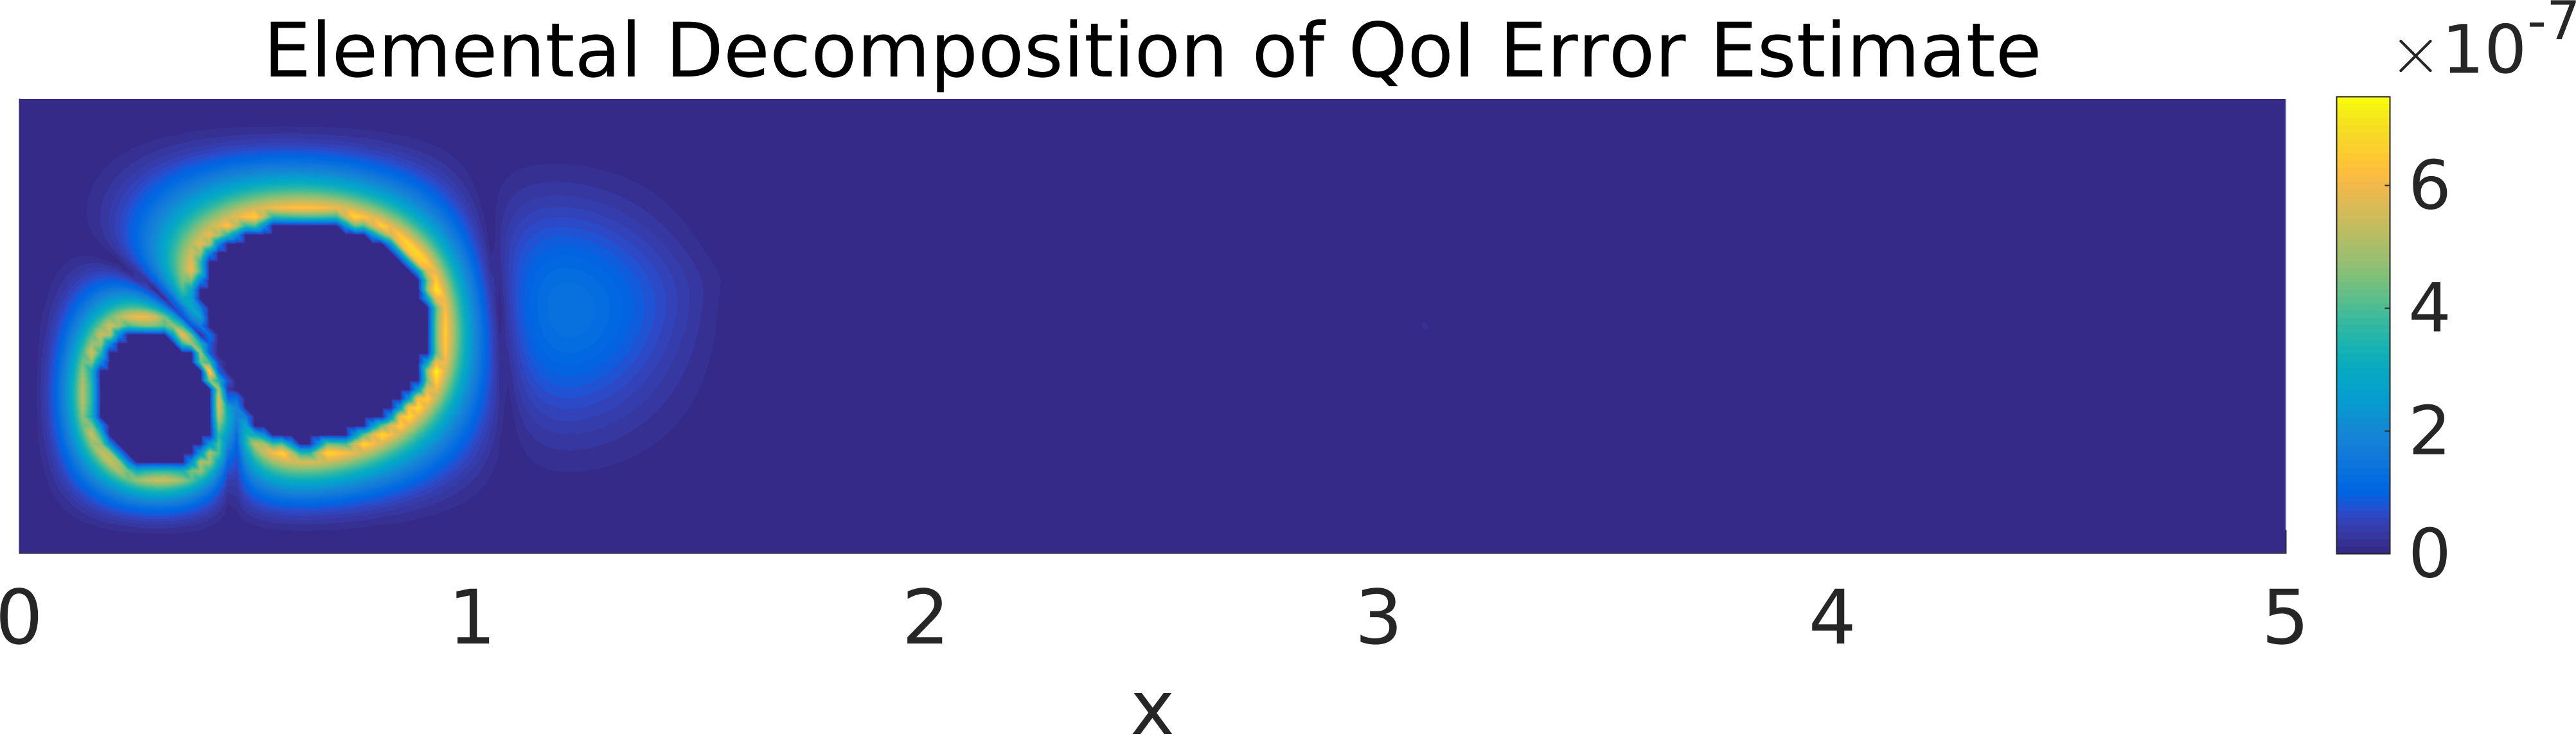
\includegraphics[width=0.49\textwidth]{svf/err_breakdown_MF01.png}
} \\
\subfloat[MF$_2$ ($20\%$ HF)]{
  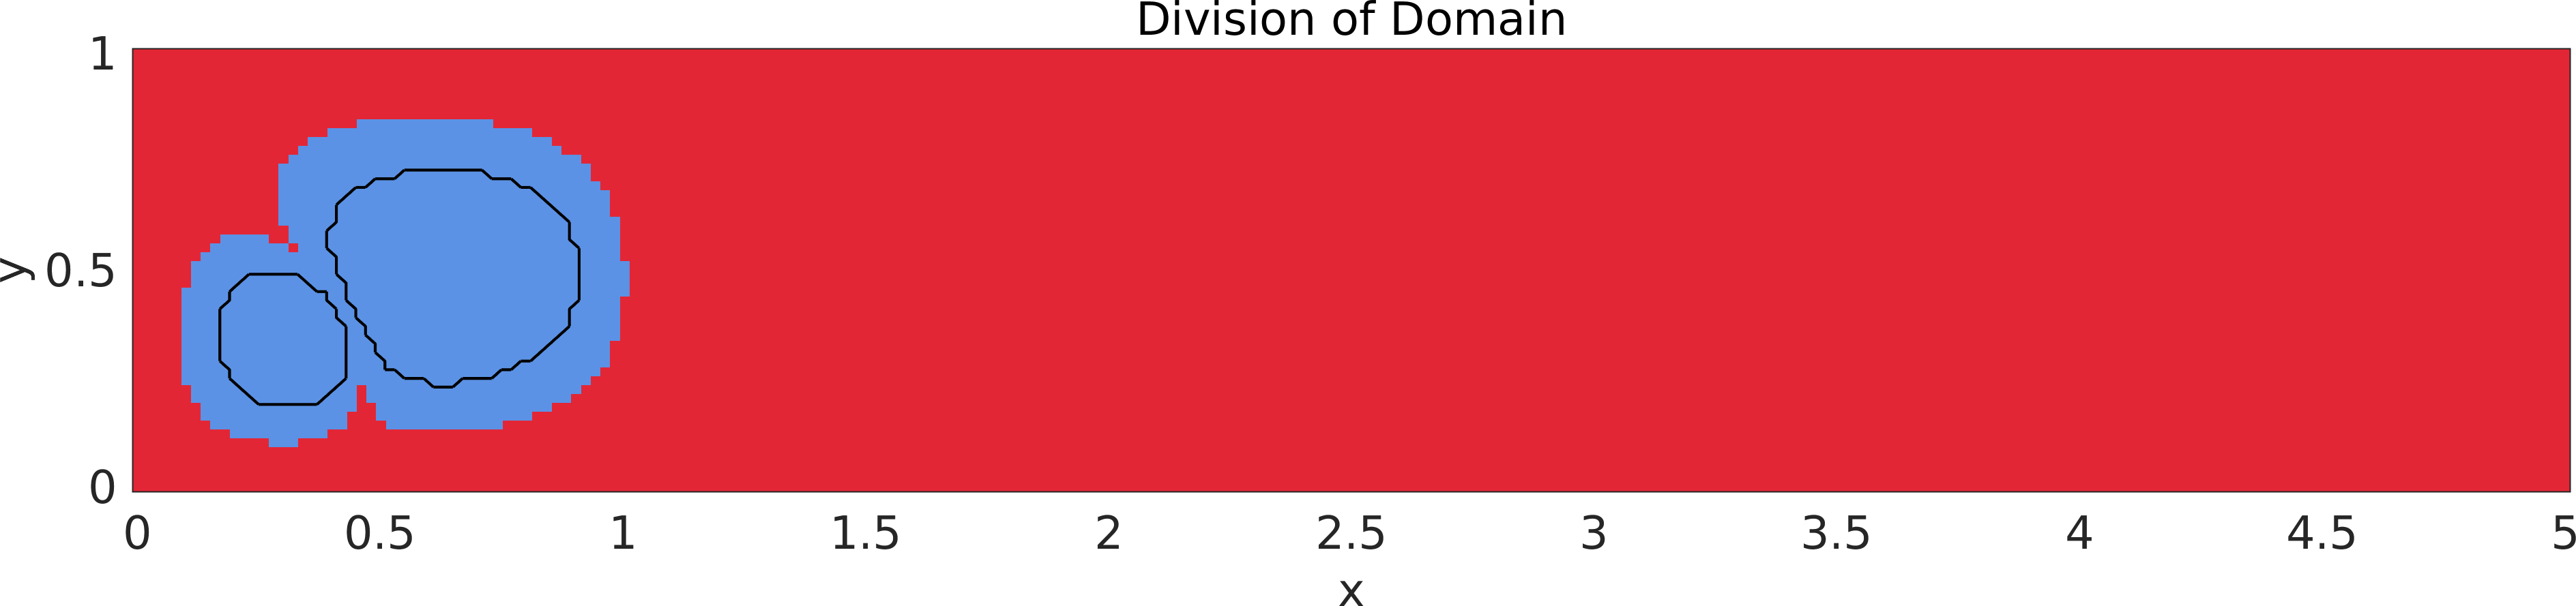
\includegraphics[width=0.46\textwidth]{svf/cd_cdr_MF02_divvy.png}
  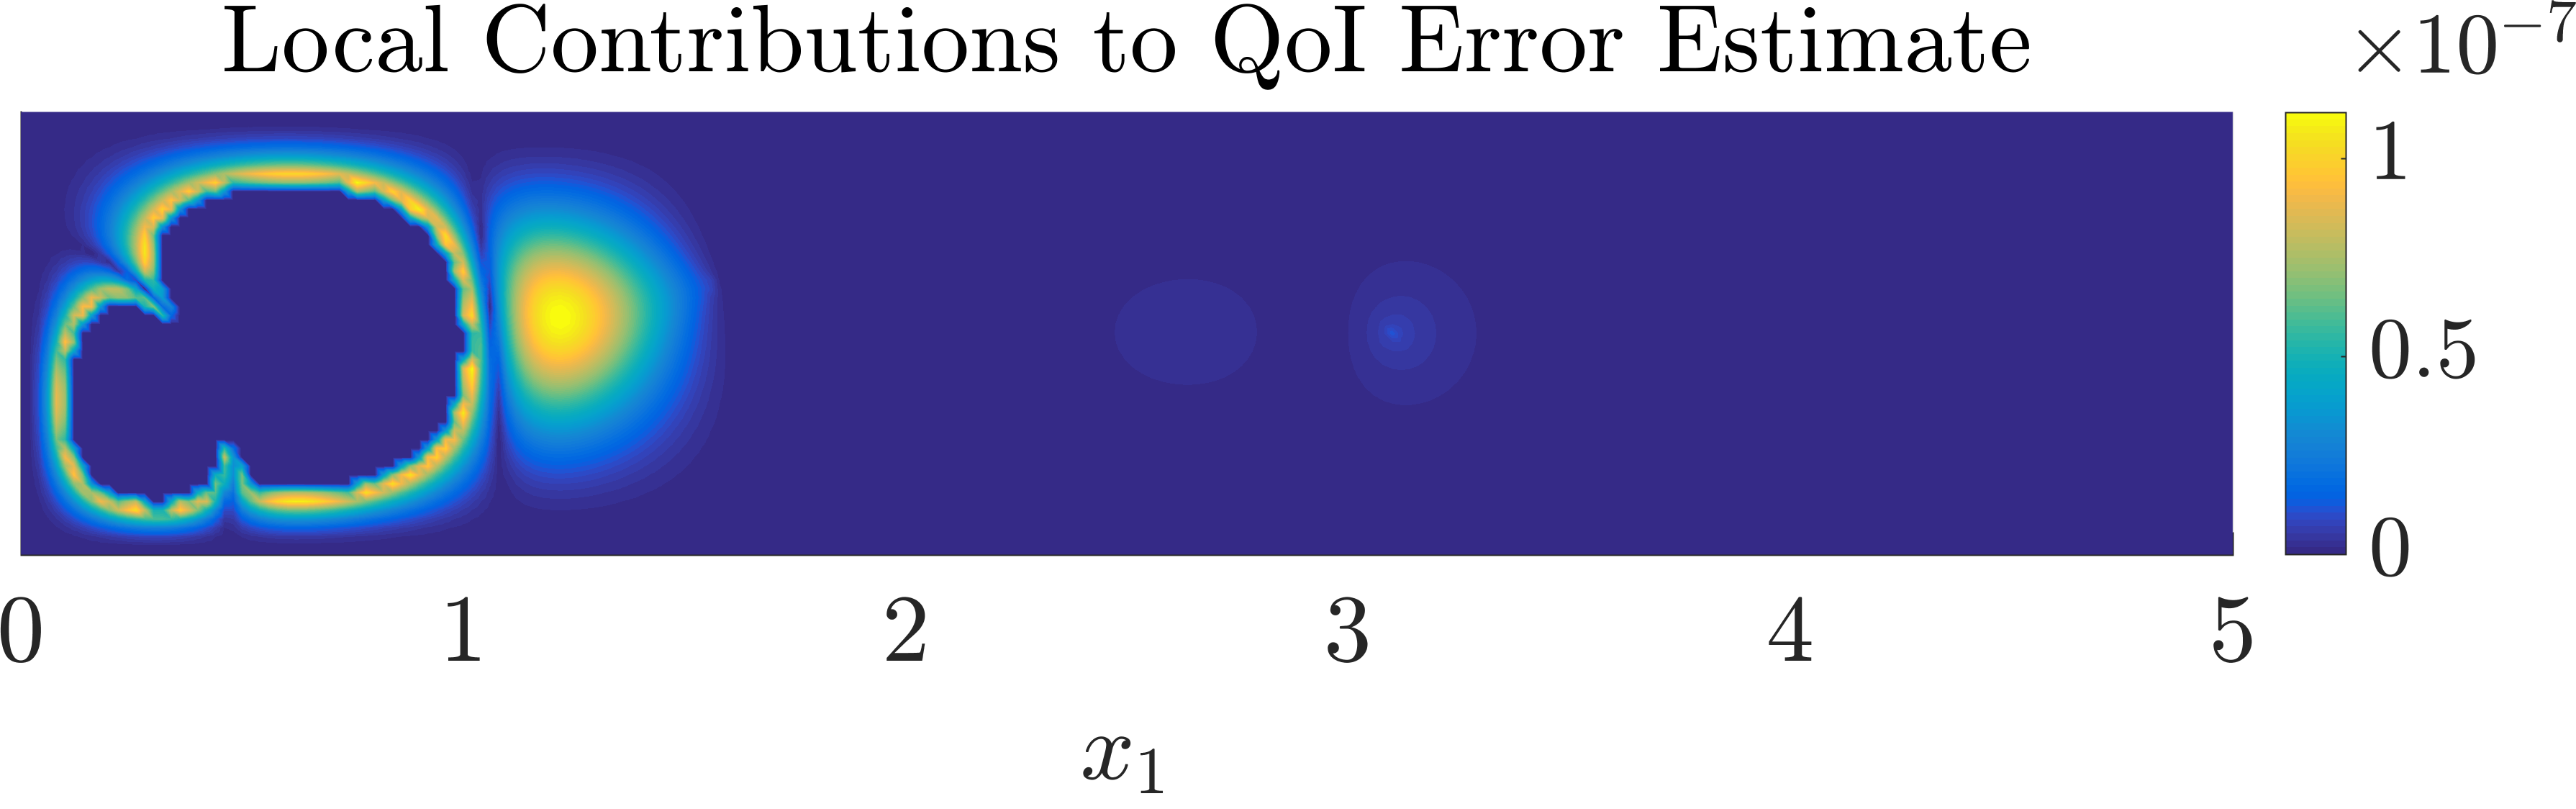
\includegraphics[width=0.49\textwidth]{svf/err_breakdown_MF02.png}
} \\
%\begin{subfigure}[b]{\textwidth}
%	\centering
%	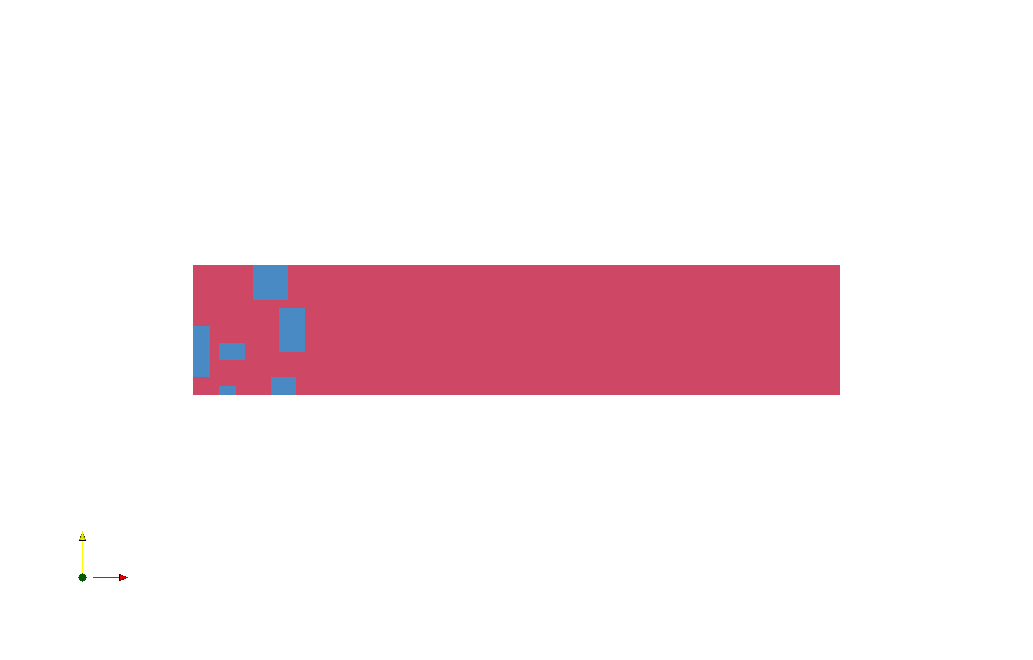
\includegraphics[width=0.48\textwidth]{svf/cd_cdr_MF03_divvy.png}
%  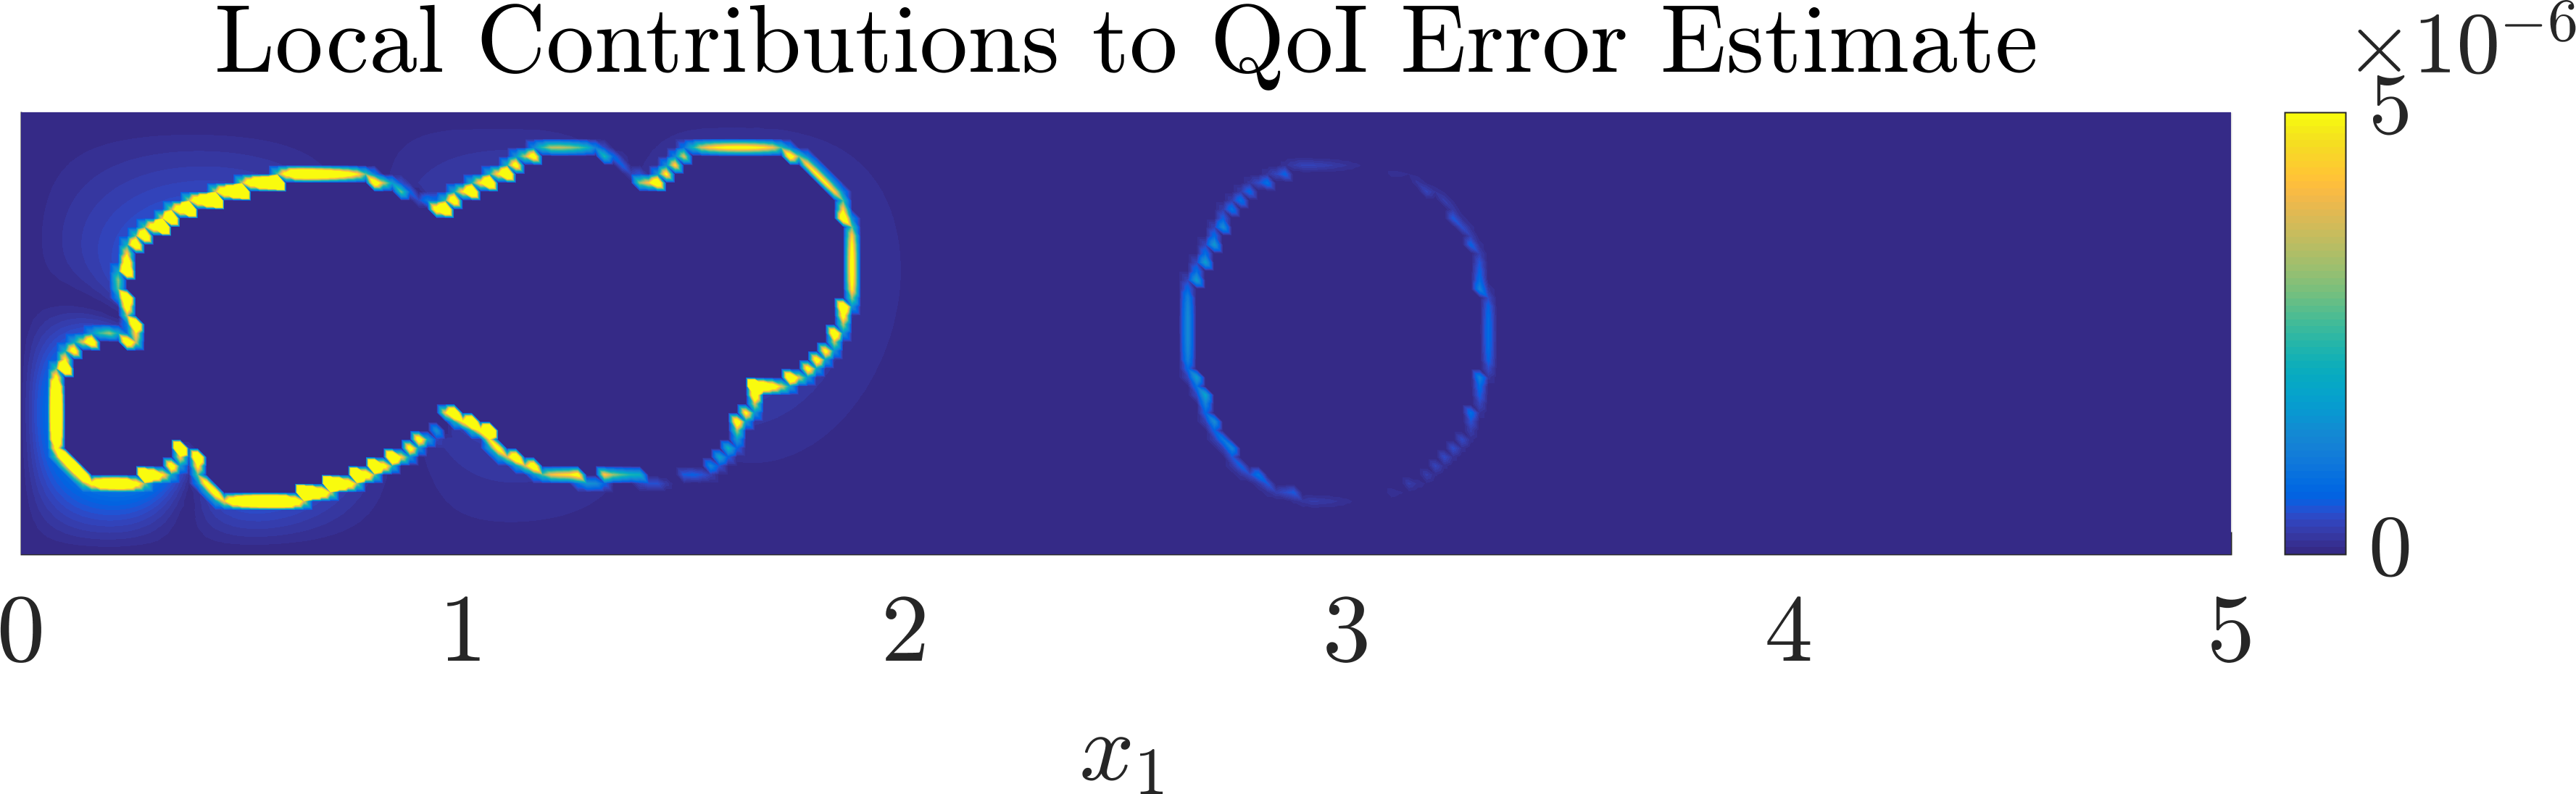
\includegraphics[width=0.51\textwidth]{svf/err_breakdown_MF03.png}
%  \vspace{-0.7\baselineskip}
%  \caption{MF$_3$ ($30\%$ HF)}
%  \vspace{0.8\baselineskip}
%\end{subfigure}
%\begin{subfigure}[b]{\textwidth}
%	\centering
%	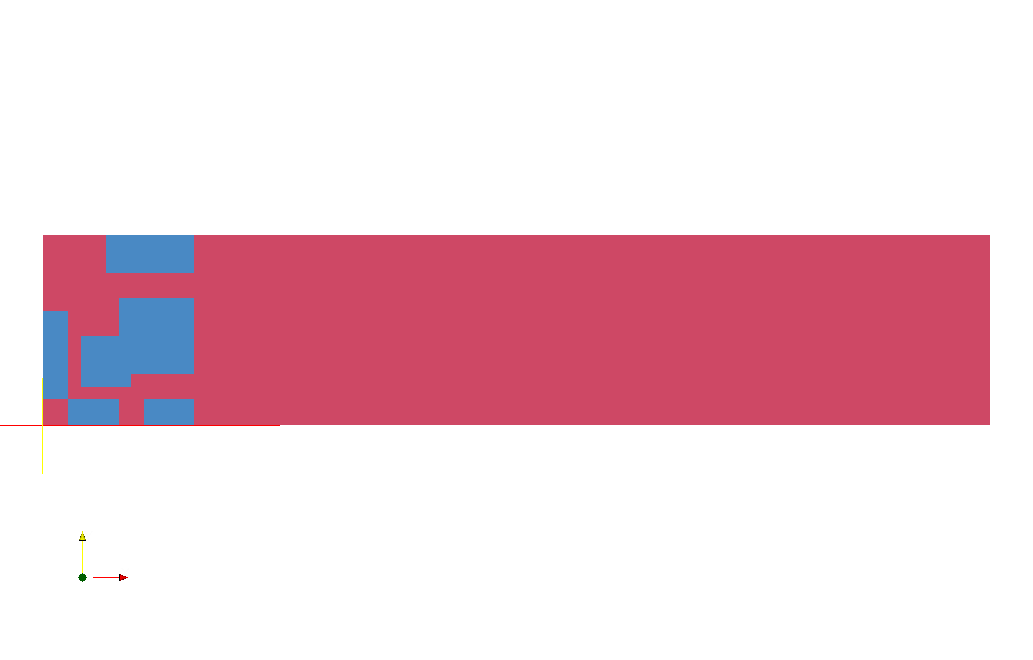
\includegraphics[width=0.48\textwidth]{svf/cd_cdr_MF04_divvy.png}
%  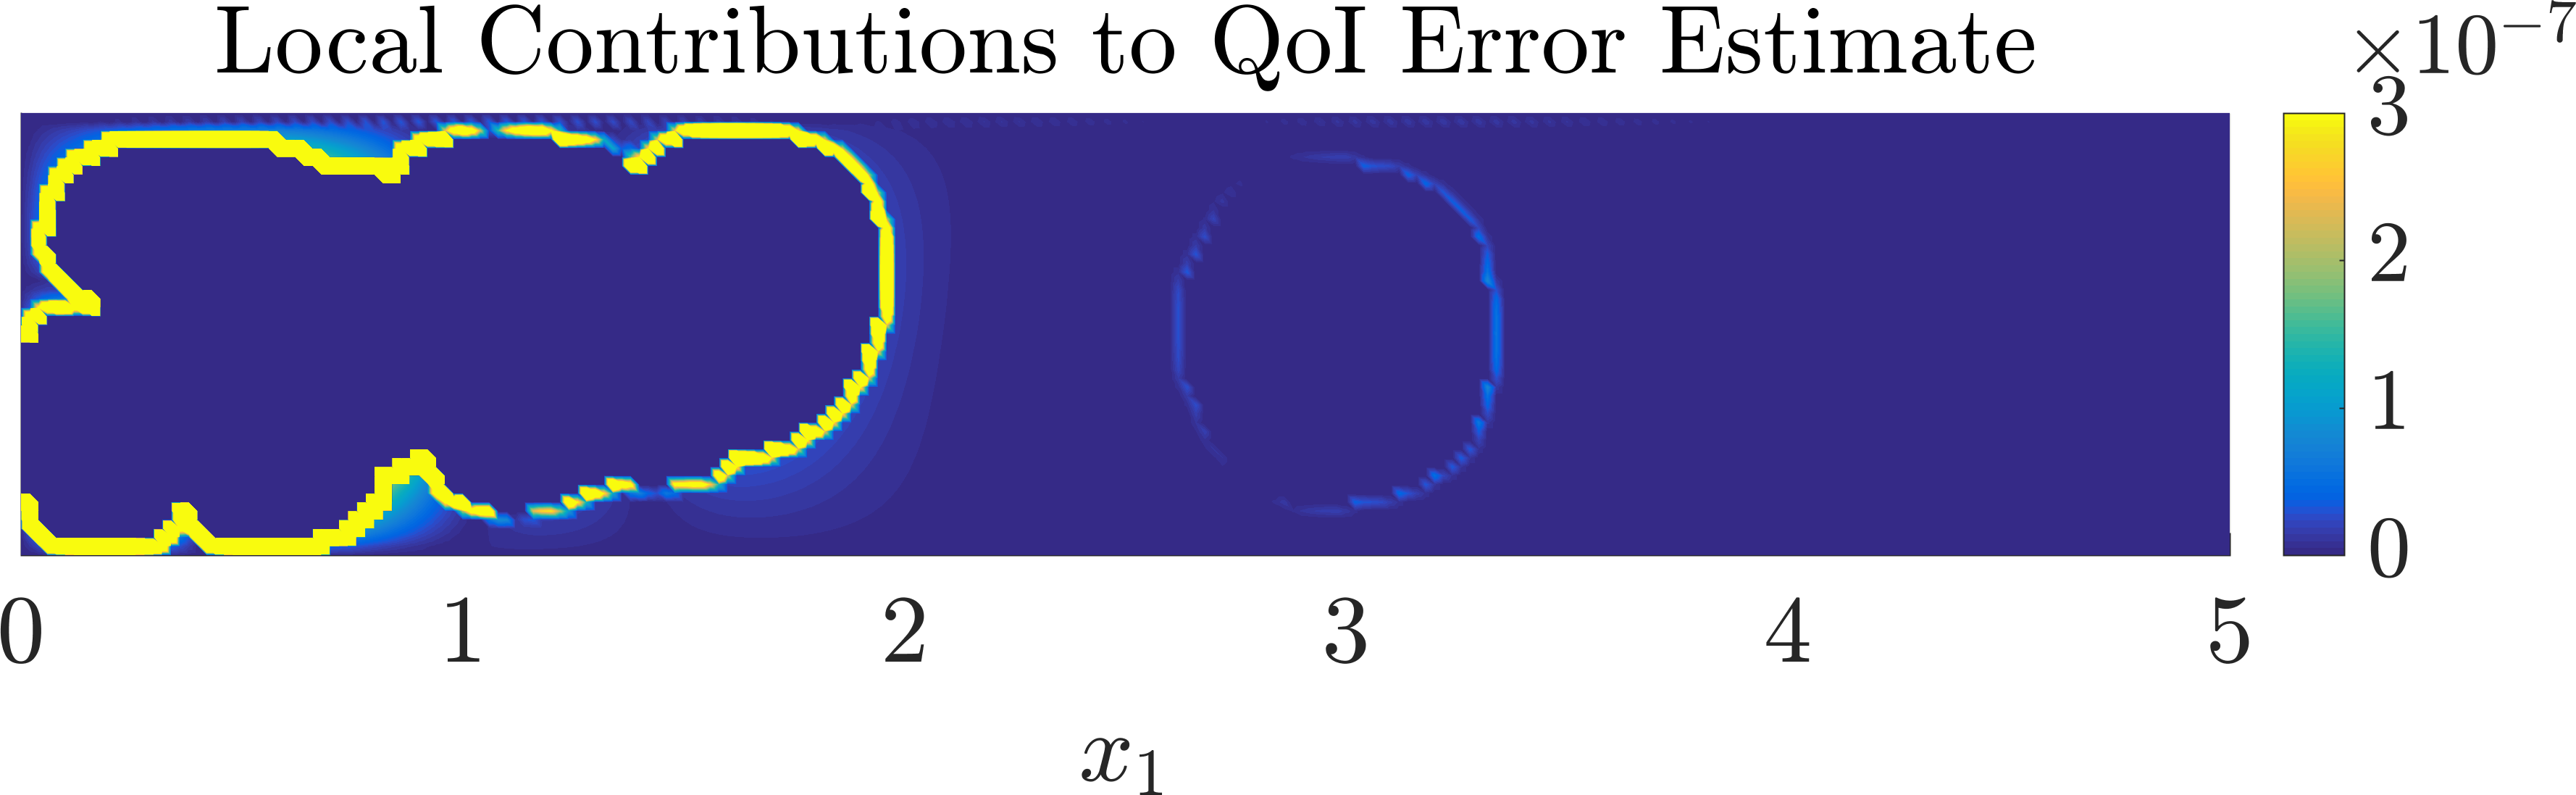
\includegraphics[width=0.51\textwidth]{svf/err_breakdown_MF04.png}
%  \vspace{-0.7\baselineskip}
%  \caption{MF$_4$ ($40\%$ HF)}
%  \vspace{0.8\baselineskip}
%\end{subfigure}
%\begin{subfigure}[b]{\textwidth}
%	\centering
%	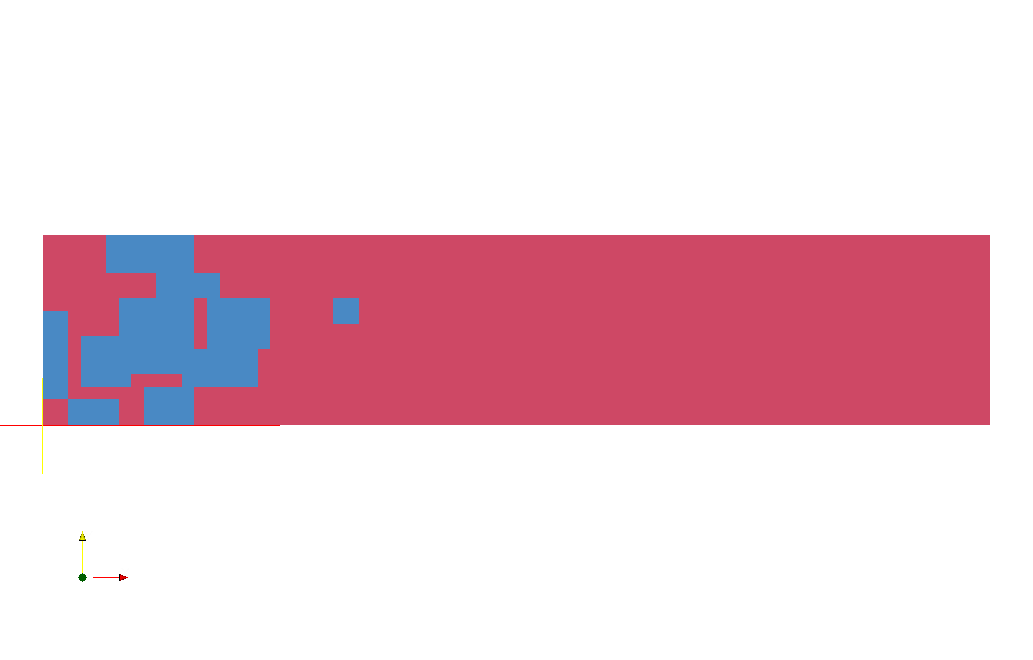
\includegraphics[width=0.48\textwidth]{svf/cd_cdr_MF05_divvy.png}
%  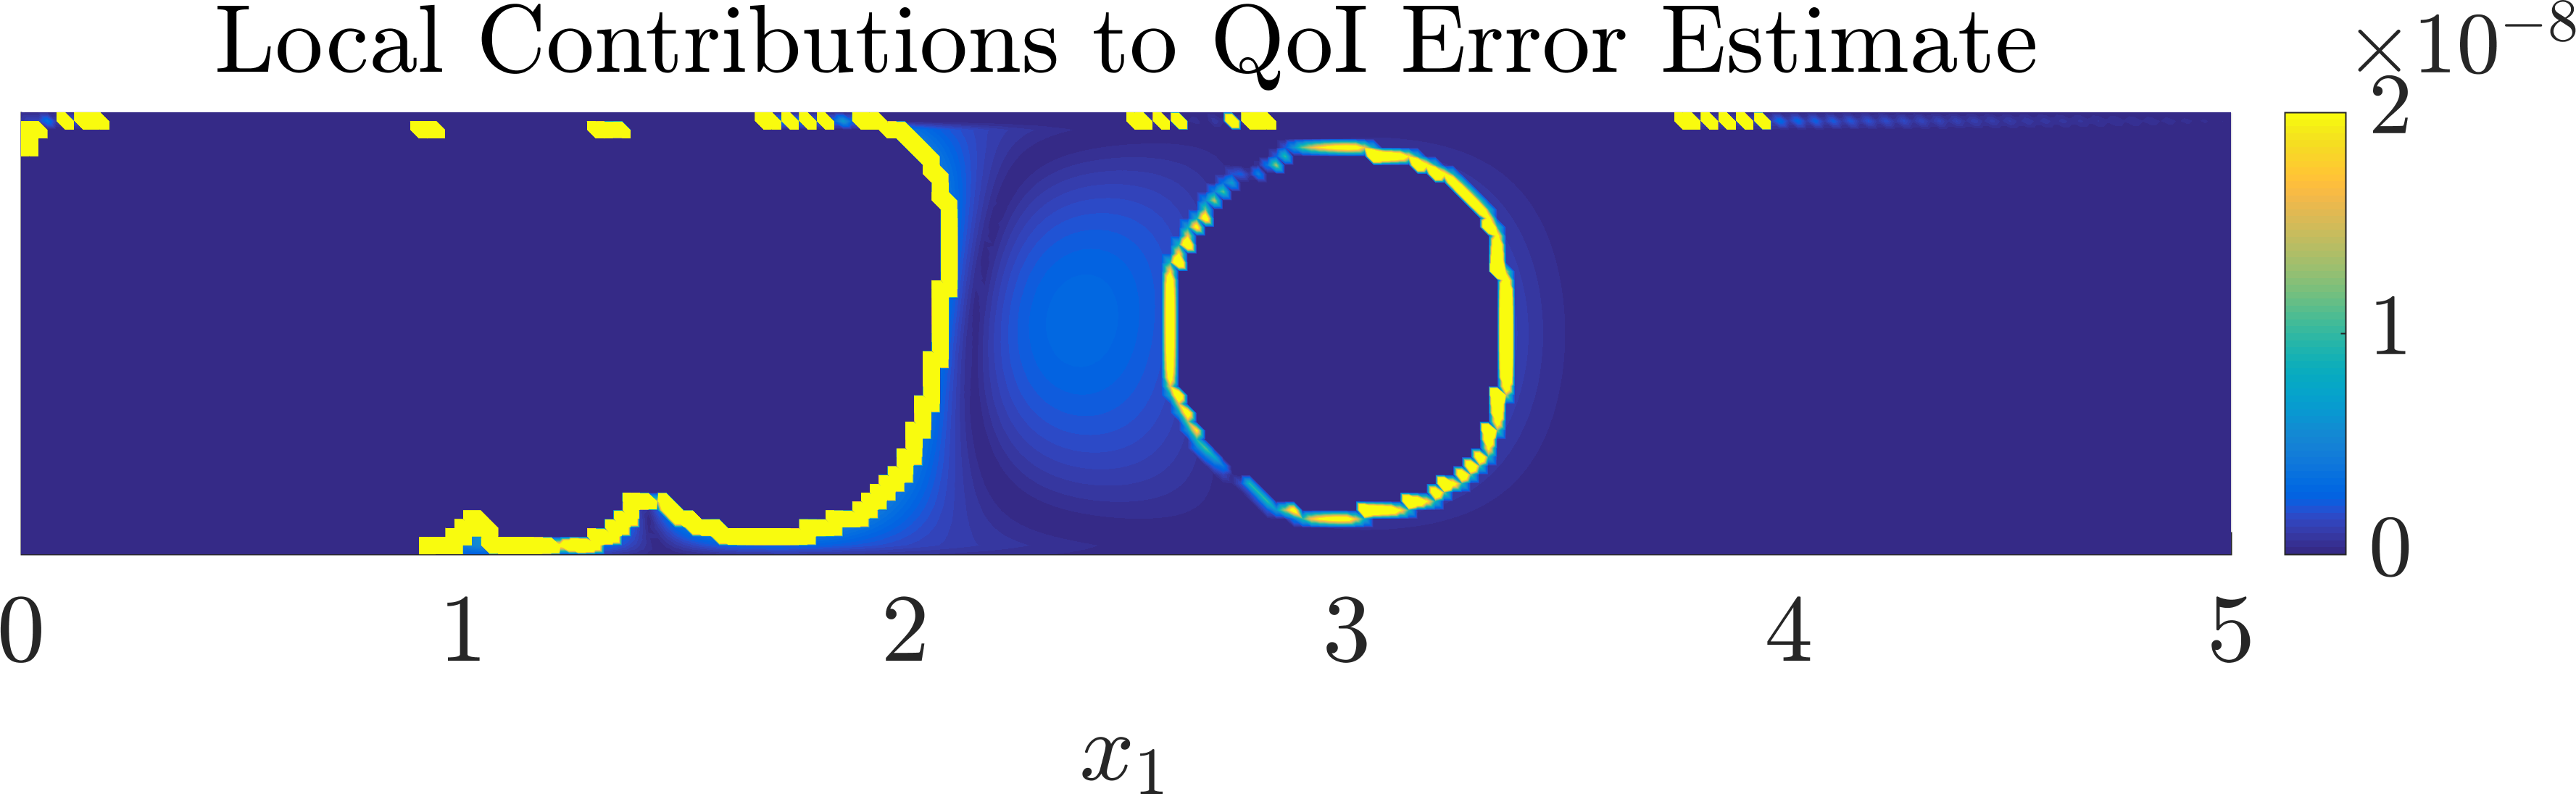
\includegraphics[width=0.51\textwidth]{svf/err_breakdown_MF05.png}
%  \vspace{-0.7\baselineskip}
%  \caption{MF$_5$ ($50\%$ HF)}
%  \vspace{0.8\baselineskip}
%\end{subfigure}
\subfloat[MF$_6$ ($60\%$ HF)]{
	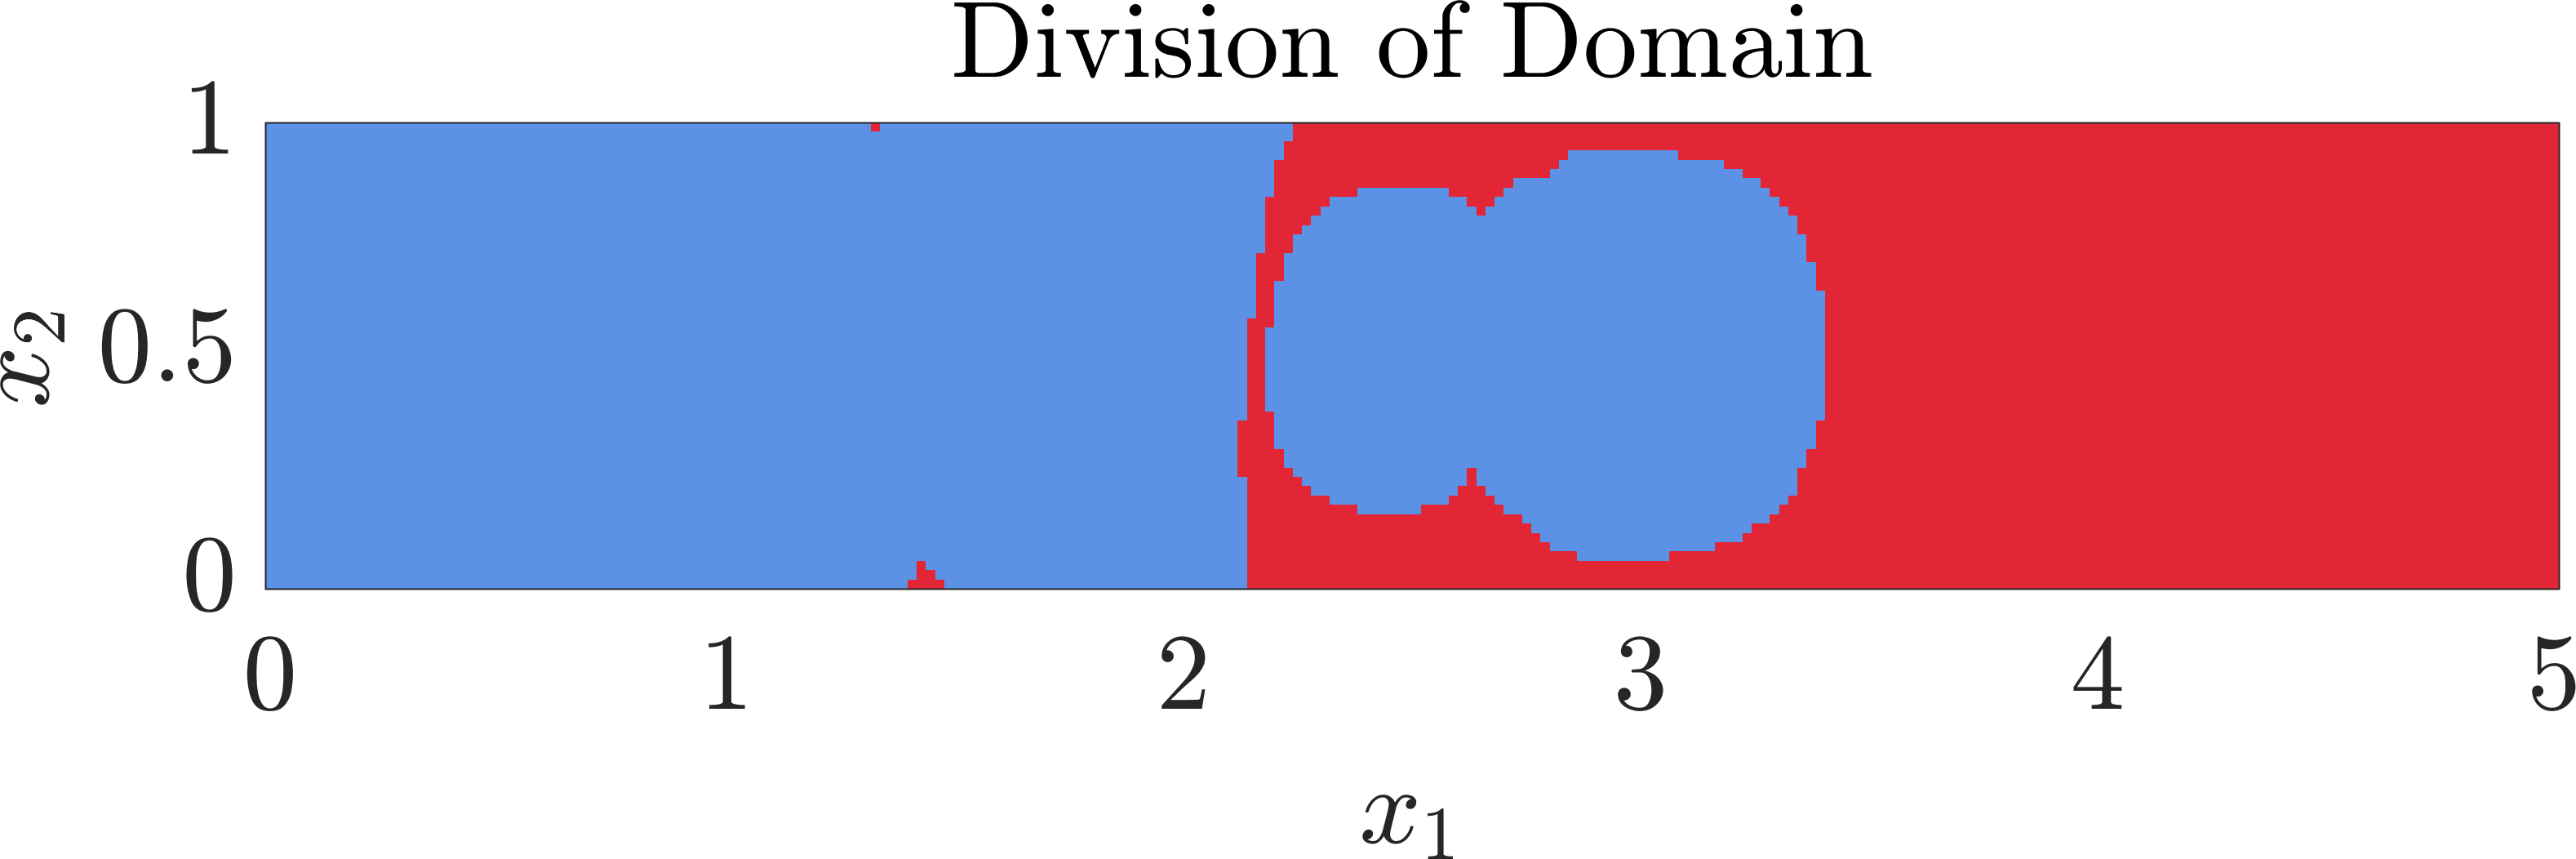
\includegraphics[width=0.46\textwidth]{svf/cd_cdr_MF06_divvy.png}
  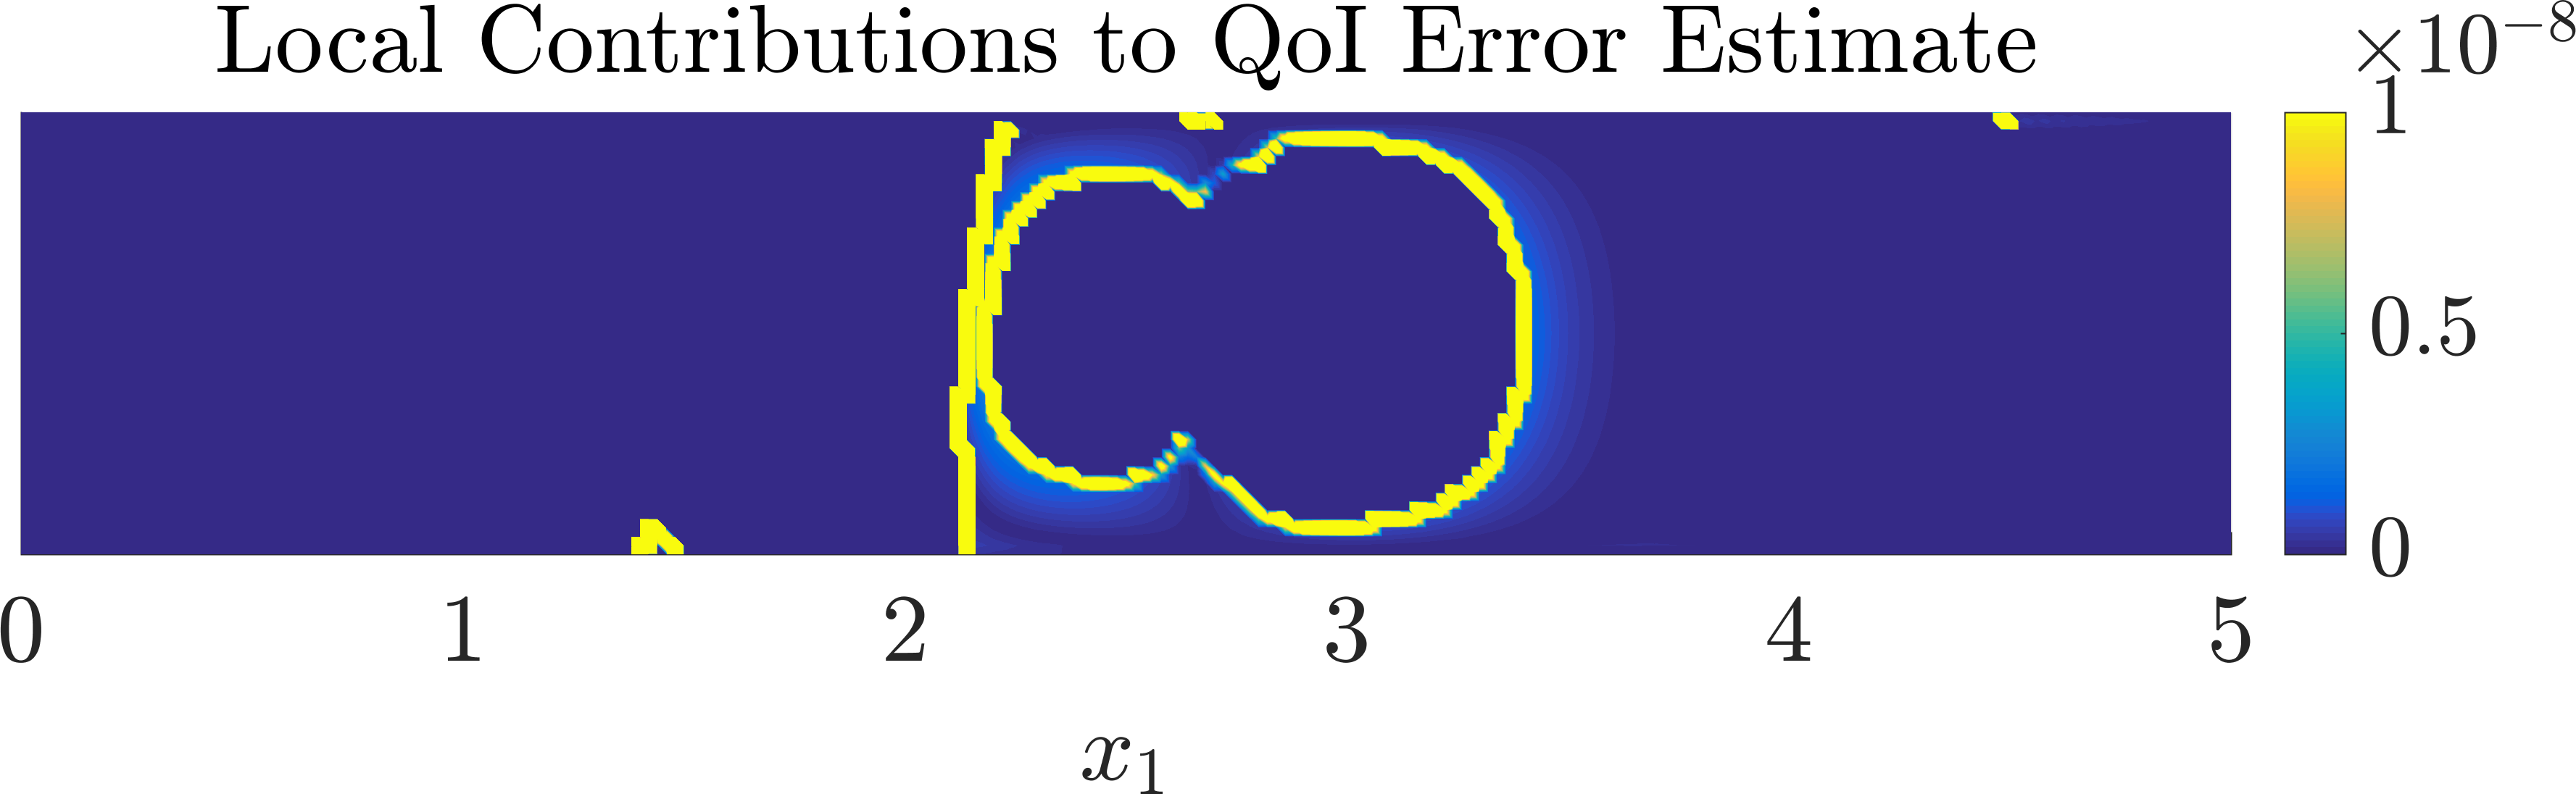
\includegraphics[width=0.49\textwidth]{svf/err_breakdown_MF06.png}
}
\caption{Local error contributions (right) and domain division (left; low-fidelity constant-parameter model used in red portion, high-fidelity field-parameter model used in blue portion) for mixed-fidelity models. The (weighted) residual, and thus the local error contribution, tends to spike sharply at the interface between the low- and high-fidelity regions; the color range is truncated to make the error distribution visible elsewhere in the domain.}
\label{fig:svfRef}
\end{figure}
%
Comparing to \cref{fig:baseRef}, we see that in this case the local error contribution is not as greatly concentrated around the QoI region and the nearest data point; here, all three data points and the QoI region have associated regions of sufficiently similar high local error that all are refined in the first iteration. This reflects the global nature of the differences between the low- and high-fidelity models; the parameter field in all the low-fidelity regions is constant and equal. 

The corresponding true and estimated absolute errors in the QoI are shown in \cref{fig:svfErr}.
%
\begin{figure}[htbp]
\centering
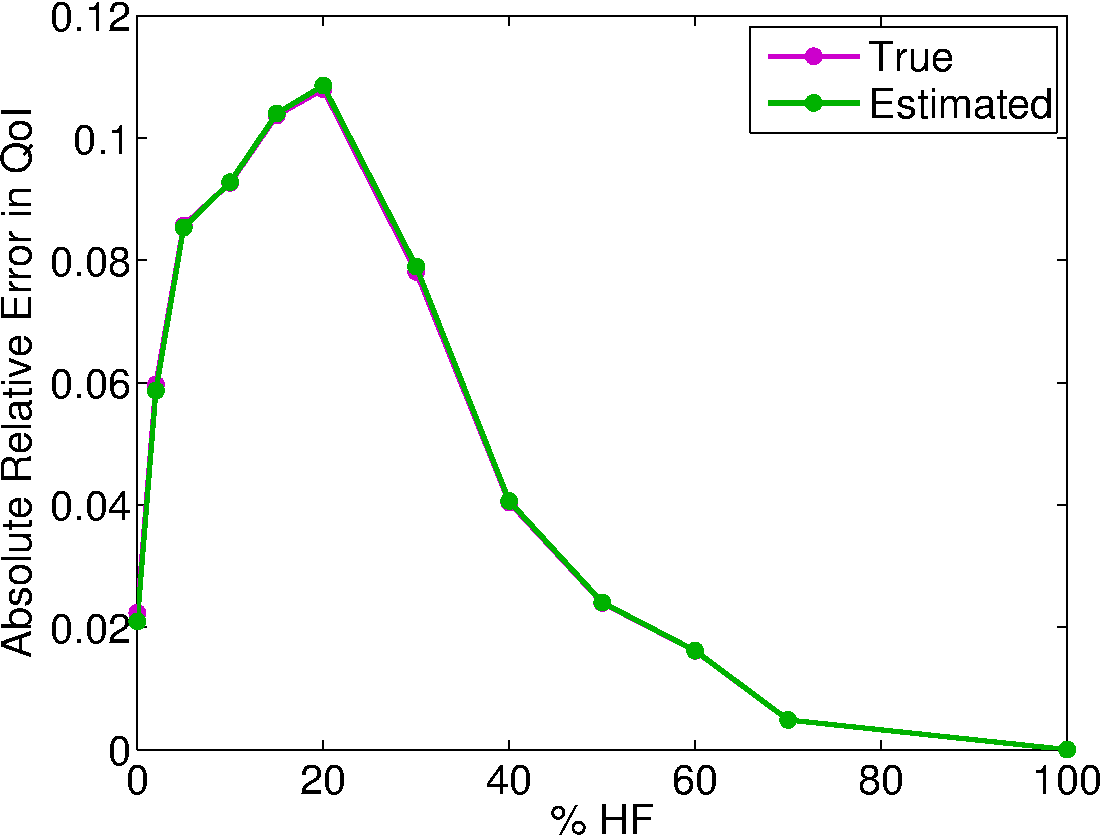
\includegraphics[width=0.8\textwidth]{svf/err_est.pdf}
\caption{True and estimated absolute relative error in QoI, plotted as a function of the percentage area of the domain in which the high-fidelity field-parameter model is used.}
\label{fig:svfErr}
\end{figure}
%
In this case, we see that we must use the high-fidelity model in most of the domain in order to get an accurate QoI. The adaptive algorithm requires us to use the field representation of the high-fidelity model in much of the left half of the domain; this reflects the topology of the inferred parameter field in the high-fidelity inverse problem, which is only relatively constant towards the right portion of the domain. We also see that in this case, compared to the example in \cref{sec:cdvcdrBaseRef}, increasing the proportion of the domain in which the high-fidelity model is used does not monotonically decrease the error in the QoI. 
%\if{0} %--*--*--*--*--*--*--*--*--*--*--*--*--*--*--*--*--*--*--*--*--*--*--*--*--*--*--*--*--*--*--
%------------------------------------------------------------------------------------------------------------------------%
\subsection{Convection-Diffusion(-Highly Nonlinear Reaction)}
%------------------------------------------------------------------------------------------------------------------------%
\red{Not sure should even keep this section...if we split the supplementary adjoint solve, then the condition for adaptivity being more efficient doesn't depend on the linear solver...we don't need this section to make a cost argument if we have the 3D example...having this section seems to be overkill/redundant if all we want to say is that 'sometimes we need continuation for the HF inverse problem'...if we want to make a 'robustness' argument, then merge with whatever vikram writes about operator continuation interpretation?

Can't seem to replicate this...in HF continuation code, going up to 1000 with steps of 100 is fine, with both gmres and superlu...perhaps there was a bug/copy-paste mistake in the manual continuation version? All notes on this run were accidentally lost, so...
%------------------------------------------------------------%
\subsubsection{Results}
%------------------------------------------------------------%

We consider the convection-diffusion-reaction term described in \cref{sec:cdvcdr}, with a reaction term $k_r=-616$ in the high-fidelity model. This reaction term is large enough that the Newton solver will not converge with a zero initial guess. We first solve the inverse problem with the low-fidelity model ($k_r=0$), and then use a simple continuation approach, using the solution at one value of $k_r$ as the initial guess for the next.\footnote{not arclength continuation, which is more difficult to implement, though libMesh appears to have a class for such continuation, which we can use if this seems like a viable direction} We increase the reaction term in increments of $\Delta k_r=100$, and halve the increment each time the step is too large (Newton solver does not converge at the next $k_r$ value). From $k_r=0$ to $k_r=-616$, this results in 9 continuation steps being taken.

%------------------------------------------------------------%
\subsubsection{Computational Complexity}
%------------------------------------------------------------%

We compare the complexity of\cref{alg:refSeries} and the continuation method for the high fidelity problem, in the context of the analysis developed in \cref{sect:alg_complexity}. For the high fidelity problem, with  with 9 continuation steps, we have $\sum\limits_{i=1}^{C} K_i=30$. 
 
With Gaussian elimination chosen as the linear solver, this gives us $T < 3$, i.e.\ a budget of 2 adaptive steps. Using \cref{alg:refSeries} with 2 refinement steps, and only $10\%$ of the domain refined to use the high-fidelity model, the estimated relative error is $<1\%$. Indeed, the ratio $\frac{C_{MF}}{C_{HF}}$ was $\frac{24}{30}$, indicating about $20\%$ reduction in computational cost, with the worst case linear solver used. 

In other words, on using \cref{alg:refSeries} for a highly nonlinear problem, even with the worst case linear solver, one can get to $<1\%$ error in the QoI, with a $20\%$ reduction in computational cost, while avoiding any need for continuation to handle nonlinearities. }

%
%
%
%
%
%
%
%

%------------------------------------------------------------------------------------------------------------------------%
\subsection{Convection-Diffusion(-Reaction) in 3D} \label{sec:cdvcdr3D}
%------------------------------------------------------------------------------------------------------------------------%

\red{In the previous examples, although the low- and high-fidelity models are sufficiently different to illustrate the behavior of \cref{alg:refSeries}, they are both simple enough and similar enough that using \cref{alg:refSeries} saves little, if any, time. In this section, we consider a more realistic pair of models which differ in the physics included, and demonstrate computational savings when using the adaptive algorithm, while still achieving a small error in the QoI. In \cref{sec:setup3D} we describe the setup of the models and their inverse problems, and in \cref{sec:ref3D} we describe the results of applying \cref{alg:refSeries} to this pair of models.}

%------------------------------------------------------------%
\subsubsection{Problem Setup} \label{sec:setup3D}
%------------------------------------------------------------%

The two models share a box domain $\Omega(x_1,x_2,x_3)$ which is $2300$m, $1650$m, and $100$m long in the $x_1$, $x_2$, and $x_3$ directions, respectively. We will refer to the positive and negative directions in $x_1$ as ``east" and ``west", respectively. The high-fidelity model is a single-species convection-diffusion-reaction equation with a nonlinear reaction term, described by
%
\begin{subequations}
\label{eq:cdvcdrHF3D}
\begin{align}
\nabla\cdot(n\vec{V}u - nD\nabla u) + k_ru^2 = f(q) \quad &\text{in } \Omega, \label{eq:HFeq3D}\\
u = 5 \quad &\text{on } \partial \Omega_{west}, \\
\frac{\partial u}{\partial n} = 0 \quad &\text{on }\partial\Omega_{east}, \\
\hat{n}\cdot(n\vec{V}u - nD\nabla u) = 0 \quad &\text{on }\partial\Omega\backslash(\partial\Omega_{east}\cup\partial\Omega_{west}),
\end{align} 
\end{subequations}
%
where the state $u$ is the mass-fraction (in parts-per-billion) of some contaminant species and $f(q)$ is a source/sink field. The velocity field is a constant $\vec{V}=(2.1,0,0)$ m/day. Given this velocity field and letting the molecular diffusion be negligble, we follow \cite{Vestedetal93} to express the (diagonal) dispersion tensor $D$ as $D_{11}=\alpha_{LH}V_1$, $D_{22}=\alpha_{TH}V_1$, and $D_{33}=\alpha_{TV}V_1$, where $\alpha_{LH}=100$m, $\alpha_{TH}=40$m, and $\alpha_{TV}=4$m are the longitudinal horizontal, transverse horizontal, and transverse vertical dispersivities, respectively; the dispersivity values were drawn from within the range of observed values in various porous media \cite{Davis86}. We have porosity $n=0.1$. The reaction coefficient is $k_r=4.2\cdot10^{-4}$ 1/day, chosen from within the wide range of reaction-rate coefficients for second-order reactions. Although the reaction term $k_ru^2$ does not correspond to any particular reaction of any particular species, we note that, in addition to second-order elementary reactions, a quadratic reaction term can appear in models of dissolution/precipitation processes in porous media \cite{Aha97} and biochemical degredation of petroleum hydrocarbons in soils \cite{Jack94}.

The low-fidelity model,
%
\begin{equation}
\nabla\cdot(n\vec{V}u - nk_d\nabla u) = f(q) \quad \text{in } \Omega, \label{eq:LFeq3D}
\end{equation}
%
differs in the removal of both the reaction term and the anisotropy of the dispersion tensor; the dispersion tensor $D$ is replaced with a scalar $k_d=D_{11}$. The boundary conditions remain unchanged. As in the previous examples in \cref{sec:cdvcdr}, the mixed-fidelity models are formed by dividing the domain into complementary subdomains $\Omega_{HF}$ and $\Omega_{LF}$, where \cref{eq:HFeq3D,eq:LFeq3D} are solved, respectively. The QoI we wish to calculate is again an integral of the state over a region $\Omega_I$. 

The unknown parameters we wish to infer correspond to the source term $f(q)=q$; we impose $f(q)=q=0$ on the boundary $\partial\Omega$. Observations at 18 points in the domain are artificially generated by running the high-fidelity model on a finer mesh. The locations of the observations as well as the QoI region $\Omega_I$ are shown in \cref{fig:setup3D}. We use a regularization term $\frac{\beta}{2}\int_\Omega \|\nabla f(q)\|_2^2\:\textrm{d}V$.
%
\begin{figure}[htbp]
\centering
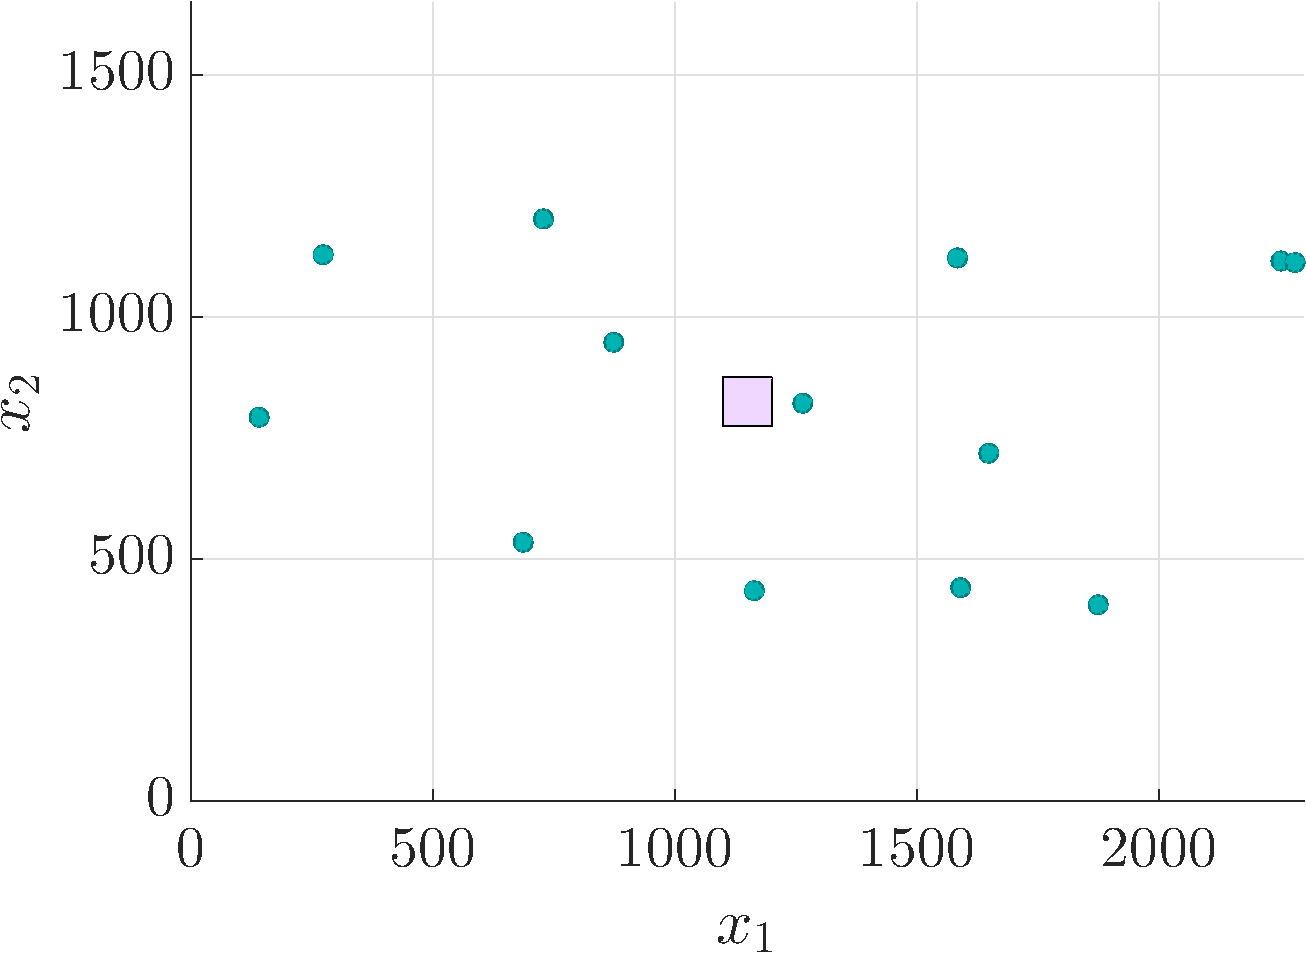
\includegraphics[width=0.4\textwidth]{series3D/setup_aerial_nolegend.pdf} \hfill
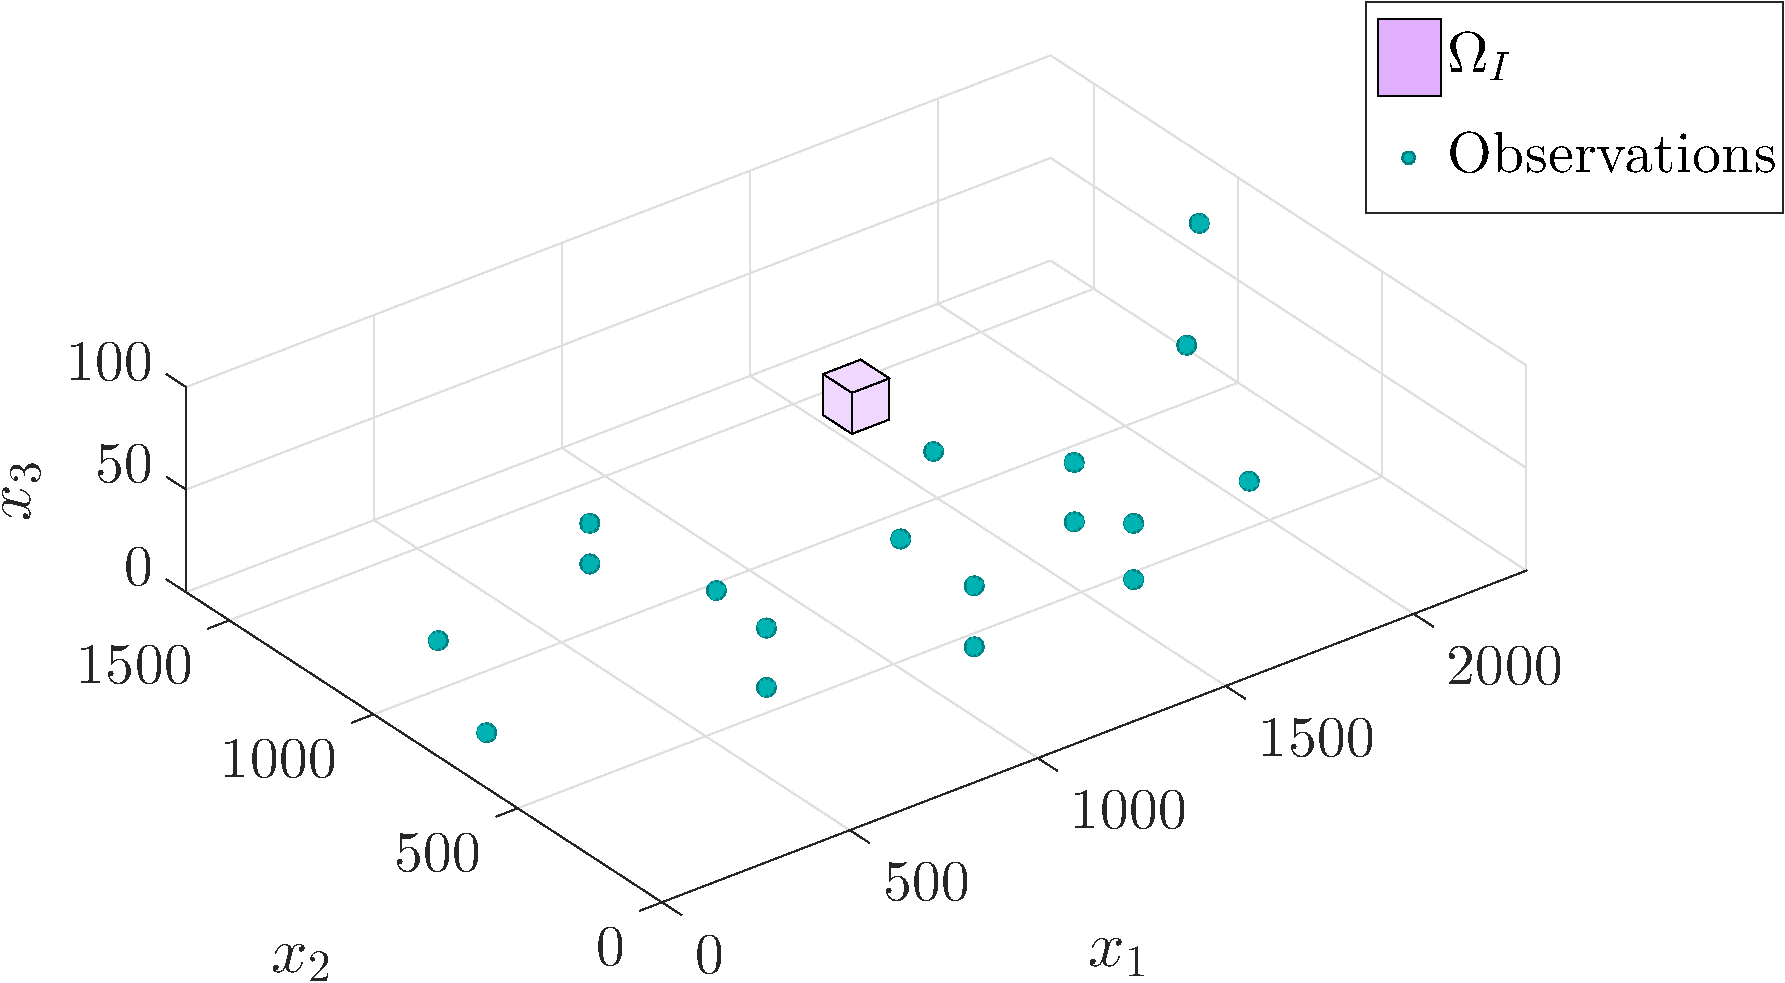
\includegraphics[width=0.55\textwidth]{series3D/setup_3view.pdf} \\ 
\vspace{\baselineskip}
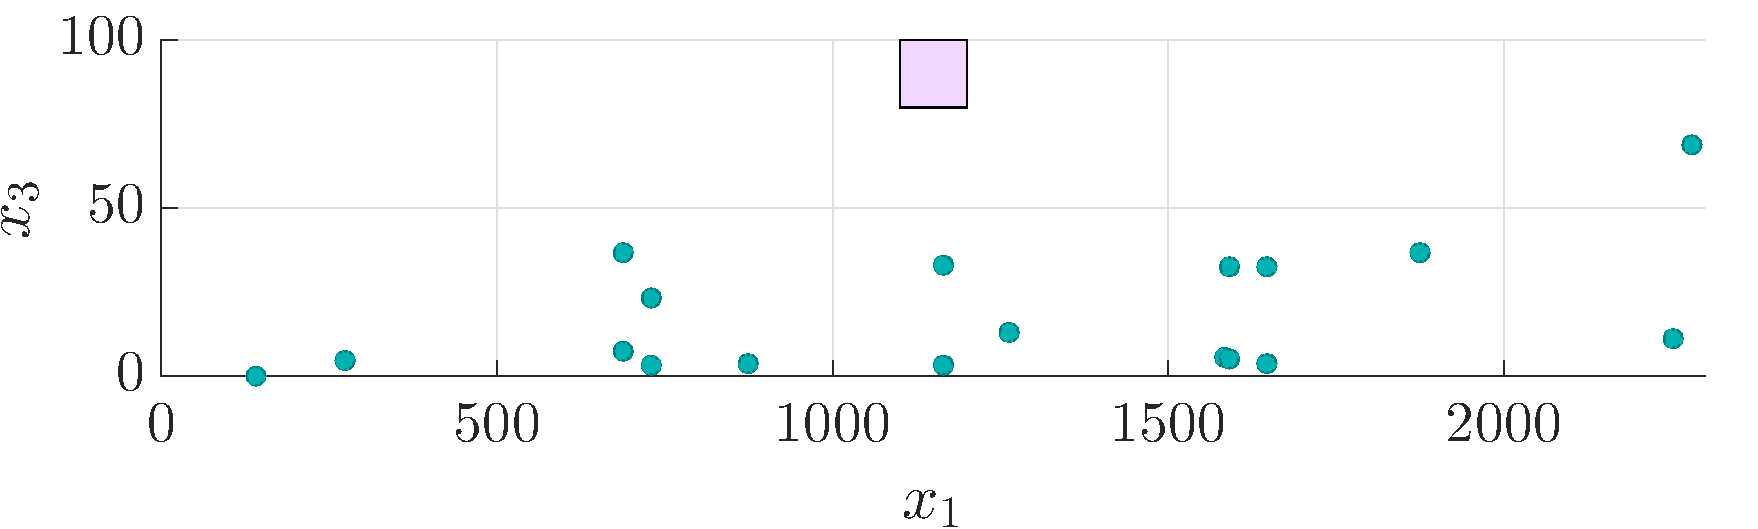
\includegraphics[width=0.6\textwidth]{series3D/setup_side_view.pdf}
\caption{Three views of the locations of the observations and the QoI region.}
\label{fig:setup3D}
\end{figure}
%
We continue to use the FEM with a continuous Galerkin formulation and Lagrange elements. The domain is discretized by a regular mesh of hexahedrons, with 25, 45, and 30 elements along the $x_1$, $x_2$, and $x_3$ directions, respectively; each variable has 37,076 degrees of freedom. The cell P\'{e}clet number is less than one and so no stabilization is used.

%------------------------------------------------------------%
\subsubsection{Adaptive Model Refinement Results} \label{sec:ref3D}
%------------------------------------------------------------%

We now present the results of solving the inference problem using \cref{alg:refSeries}, with a relative error tolerance of $1\%$. At each iteration, we choose the $5\%$ of the basis functions with the largest error for model refinement; since each linear Lagrange basis function has eight elements in its support, the number of additional elements marked for refinement in each iteration may be greater. All simulations are run on a single processor; we use the default nonlinear solver in \texttt{libMesh} (Newton's method with Brent line-search), and linear solves are performed using PETSC's GMRES solver, preconditioned by incomplete factorization. \Cref{tab:ref3D} shows the error at the end of each adaptive iteration. The high-fidelity inverse problem is solved by using natural continuation on the reaction parameter to avoid stalling the Newton iterations; only two steps are required: $k_r=0$, then $k_r=4.2\cdot10^{-4}$. Each iteration of the adaptive algorithm uses the solution of the previous iteration as its initial guess. 
%
\begin{table}[htbp]
\caption{Runtime and relative errors of adaptive algorithm iterations given relative error tolerance of $1\%$; relative errors are given with respect to the true high-fidelity QoI.}
\label{tab:ref3D}
\centering
\begin{tabular}{|c|c|c|c|c|c|c|}
\hline
\multirow{2}{*}{Case} & \multirow{2}{*}{$\%$HF} & \multirow{2}{*}{QoI} & Error & Error & $\%$ Relative \\ 
& & & (Estimated) & (Actual) & Error (Actual) \\ \hline
LF   & 0    & 133730 & -4024 & -6020 & -4.71  \\
MF01 & 10.0 & 125073 & 4404  & 2637  & 2.06   \\
MF02 & 17.7 & 123093 & 6761  & 4617  & 3.62   \\
MF03 & 25.0 & 123460 & 6354  & 4250  & 3.33   \\
MF04 & 32.9 & 125291 & 2242  & 2419  & 1.89   \\
MF05 & 39.7 & 126314 & 2445  & 1396  & 1.09   \\
MF06 & 47.2 & 126927 & 1070  & 783   & 0.61   \\
HF   & 100  & 127710 & --    & --     & --    \\ \hline
\end{tabular}
\end{table}
%

Compared to the previous examples in \cref{sec:cdvcdr} with similar physics in the pair of models, we observe that the error in the QoI (both true and estimated) does not decrease monotonically as the percentage of the domain in which the high-fidelity model is used increases. We also observe that any oscillations tend to occur within the first few iterations; continuing the adaptive algorithm beyond those iterations shown in \cref{tab:ref3D} monotonically decreases the QoI errors with increased refinement, until the high-fidelity model is used in the entire domain.

The domain divisions for the six adaptive iterations are shown in \cref{fig:divvy3D}. We see that the error decomposition causes the first refinement iteration to target the QoI region and observations; similarly to the behavior seen in \cref{sec:cdvcdrBaseRef}, those measurement points furthest downstream of the QoI region are refined later. Around the QoI region, the first iteration refines the domain completely in the $x_3$ direction, possibly reflecting the large difference in the high-fidelity dispersion tensor $D$ and the low-fidelity dispersion coefficient in the $x_3$ direction.
%
\begin{figure}[htbp]
\centering
\subfloat[MF$_1$]{
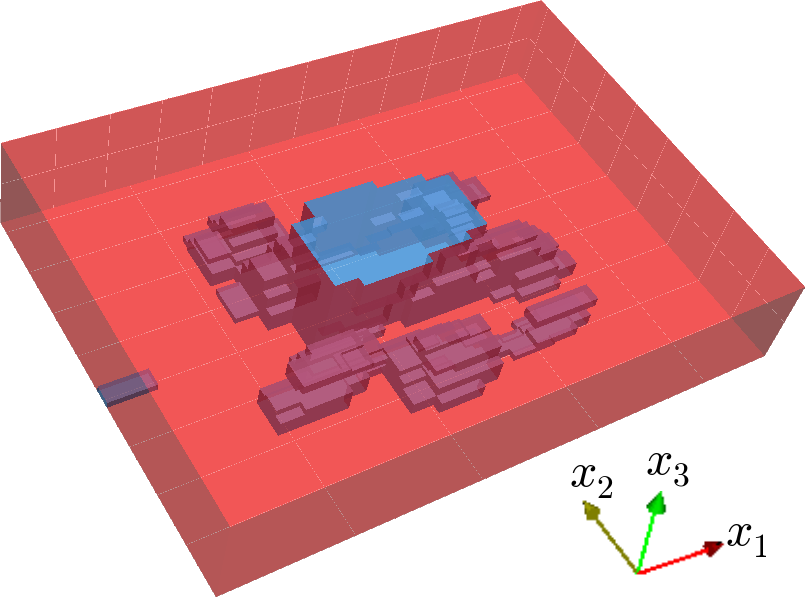
\includegraphics[width=0.31\textwidth]{series3D/run_invcrime/divvy1_whitebg_puff.png} 
}
\subfloat[MF$_2$]{
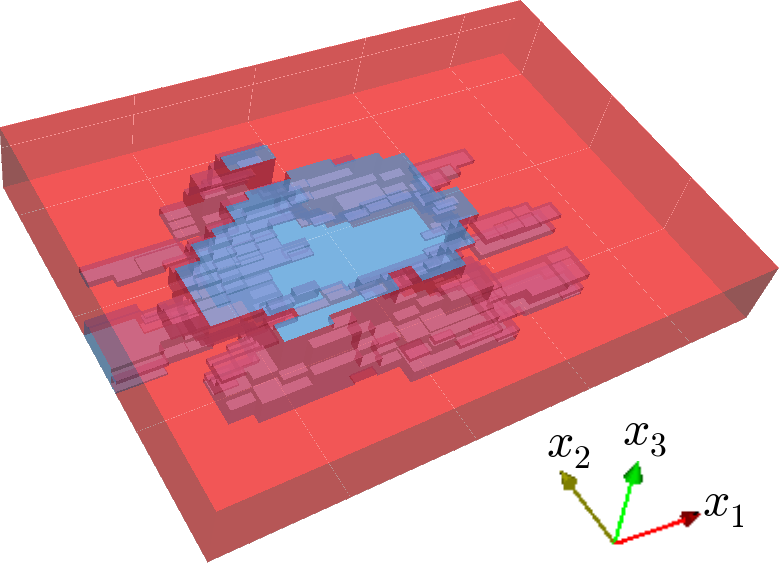
\includegraphics[width=0.31\textwidth]{series3D/run_invcrime/divvy2_whitebg_puff.png} 
}
\subfloat[MF$_3$]{
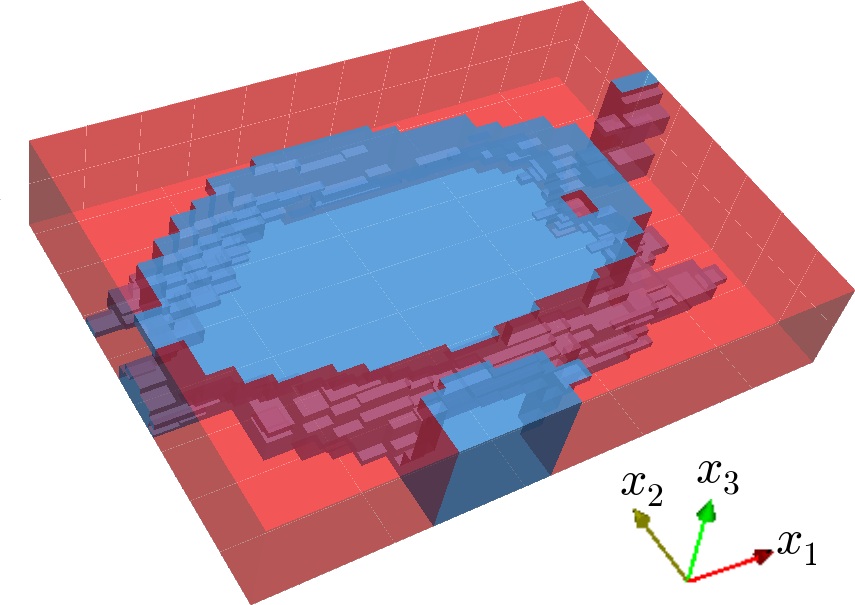
\includegraphics[width=0.31\textwidth]{series3D/run_invcrime/divvy3_whitebg_puff.png} 
} \\
\subfloat[MF$_4$]{
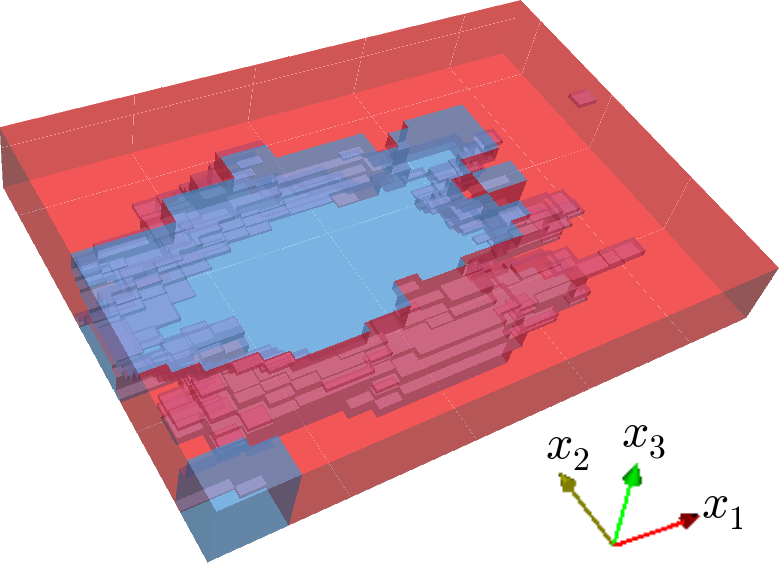
\includegraphics[width=0.31\textwidth]{series3D/run_invcrime/divvy4_whitebg_puff.png} 
}
\subfloat[MF$_5$]{
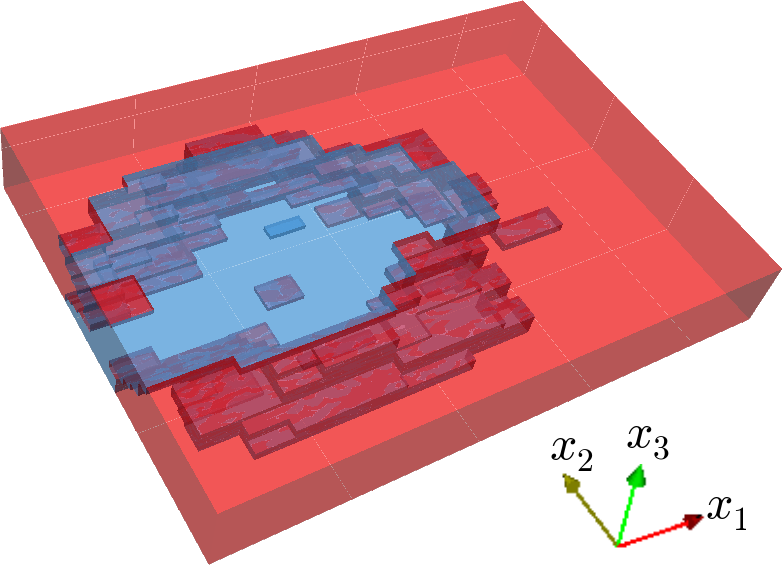
\includegraphics[width=0.31\textwidth]{series3D/run_invcrime/divvy5_whitebg_puff.png} 
}
\subfloat[MF$_6$]{
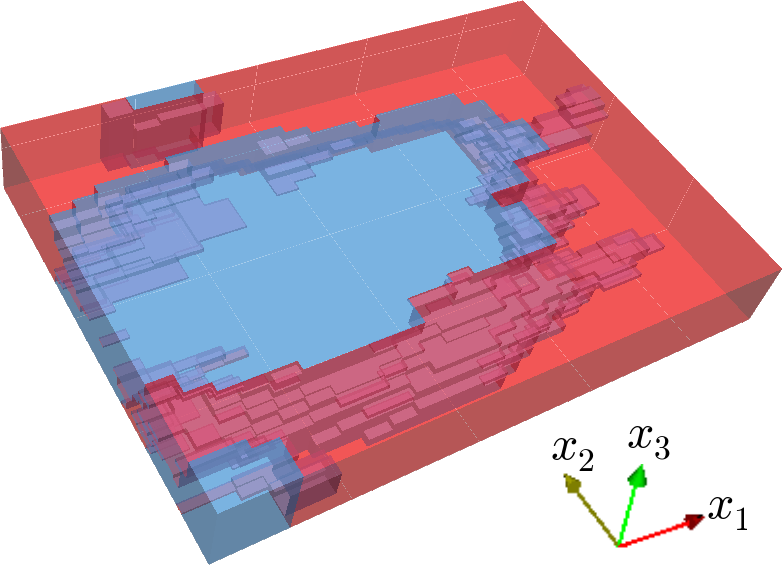
\includegraphics[width=0.31\textwidth]{series3D/run_invcrime/divvy6_whitebg_puff.png} 
}
\caption{Domain division for mixed-fidelity models: low-fidelity convection-diffusion model used in red portion, high-fidelity convection-diffusion-reaction model used in blue portion (intermediate colors due to transparency indicate a mix of the two models along the line of sight); $x_3$ direction scaled for clarity.}
\label{fig:divvy3D}
\end{figure} 
%

In this case, the high-fidelity inverse problem is only mildly nonlinear and requires few continuation steps and Newton iterations to converge; there are no savings in computational time from using the adaptive algorithm instead of solving the high-fidelity inverse problem. However, one would expect solving the high-fidelity inverse problem to require more time relative to using the adaptive algorithm as the nonlinearity of the high-fidelity model increases. 

\Cref{alg:refSeries} is also ammenable to an offline-online decomposition, analagous to that proposed in \cite{LiebWill13}. The offline phase would consist of adaptively creating a mixed-fidelity model with an appropriate error tolerance given some expected observations $d^*$. When new data is received, one can then solve the inverse problem with the chosen mixed-fidelity model and the new data, and, if desired, compute an error estimate for the QoI. The mixed-fidelity inverse problems can be expected to require less time to solve than the high-fidelity inverse problems.

To illustrate the offline-online application, we generate ten sets of noisy observations to represent the new data gained during the online phase; the noisy observations are generated by taking the observations used in the adaptive algorithm and adding Gaussian white noise with standard deviation of $\sigma=0.05$ (equivalent to anywhere from $1.7\%$ to $17\%$ of the observed values). We then solve the inverse problem using each of the mixed-fidelity models depicted in \cref{tab:ref3D,fig:divvy3D} as well as the high-fidelity model. The high-fidelity inverse problem is solved using the same two continuation steps; the first continuation step is also used as an initial guess for the mixed-fidelity inverse problems. The auxiliary and supplementary adjoint variables simply have a zero initial guess. \Cref{tab:ref3D_newdata_QoI,tab:ref3D_newdata_times} shows the average QoI values and error estimates and solution times over the ten datasets.
%
\begin{table}
\caption{Average QoI values and errors from solving inverse problem with mixed- and high-fidelity models and noisy data; relative errors are with respect to true high-fidelity QoI.}
\label{tab:ref3D_newdata_QoI}
\centering
\begin{tabular}{|c|c|c|c|c|c|}
\hline
\multirow{2}{*}{Case} & \multirow{2}{*}{$\%$HF} & \multirow{2}{*}{QoI} & Error & Error & $\%$ Relative  \\ 
& & & (Estimated) & (Actual) & Error (Actual) \\ \hline
LF   & 0.0  &  &  &  &  \\
MF01 & 10.0 & 123672 & 4328 & 2599 & 2.08  \\
MF02 & 17.7 & 122073 & 6331 & 4197 & 3.34  \\
MF03 & 25.0 & 122409 & 5972 & 3861 & 3.06  \\
MF04 & 32.9 & 124011 & 3449 & 2260 & 1.79  \\
MF05 & 39.7 & 124852 & 2481 & 1418 & 1.12  \\
MF06 & 47.2 & 125440 & 1123 & 830  & 0.66  \\ 
HF   & 100  & 126270 & --   & --   & --     \\ \hline
\end{tabular}
\end{table}
%
\begin{table}
\caption{Average times to solve inverse problem and obtain error estimate with mixed- and high-fidelity models and noisy data.}
\label{tab:ref3D_newdata_times}
\centering
\begin{tabular}{ccc|c|c|c}
\cline{4-5} 
 & & & \multicolumn{2}{|c|}{Error Estimation} & \\
\cline{1-6}
\multicolumn{1}{|c|}{\multirow{3}{*}{Case}} & \multicolumn{1}{|c|}{\multirow{3}{*}{$\%$HF}} & Inverse & Auxiliary & Supplementary & \multicolumn{1}{|c|}{Total} \\
\multicolumn{1}{|c|}{} & \multicolumn{1}{|c|}{} & Problem & Variables & Adjoint & \multicolumn{1}{|c|}{Solution}\\
\multicolumn{1}{|c|}{} & \multicolumn{1}{|c|}{} & Time (s) &  Time (s) & Time (s) & \multicolumn{1}{|c|}{Time (s)}\\
\cline{1-6}
\multicolumn{1}{|c|}{LF}    & \multicolumn{1}{|c|}{0.0}   &  &  &  & \multicolumn{1}{|c|}{} \\ \hline
\multicolumn{1}{|c|}{MF01}  & \multicolumn{1}{|c|}{10.0}  & 173 & 48 & 103 & \multicolumn{1}{|c|}{323} \\ \hline
\multicolumn{1}{|c|}{MF02}  & \multicolumn{1}{|c|}{17.7}  & 191 & 49 & 104 & \multicolumn{1}{|c|}{343} \\ \hline
\multicolumn{1}{|c|}{MF03}  & \multicolumn{1}{|c|}{25.0}  & 192 & 51 & 109 & \multicolumn{1}{|c|}{352} \\ \hline
\multicolumn{1}{|c|}{MF04}  & \multicolumn{1}{|c|}{32.9}  & 190 & 49 & 96  & \multicolumn{1}{|c|}{334} \\ \hline
\multicolumn{1}{|c|}{MF05}  & \multicolumn{1}{|c|}{39.7}  & 188 & 49 & 92  & \multicolumn{1}{|c|}{329} \\ \hline
\multicolumn{1}{|c|}{MF06}  & \multicolumn{1}{|c|}{47.2}  & 189 & 50 & 89  & \multicolumn{1}{|c|}{327} \\ \hline
\multicolumn{1}{|c|}{HF}    & \multicolumn{1}{|c|}{100}   & 214 & -- & --  & \multicolumn{1}{|c|}{214} \\ \hline
\end{tabular}
\end{table}
%

We see that in this case, when the mixed-fidelity models are used to infer from observations different from those they were generated with, they continue to give similar relative accuracy in their QoI. We also note that the mixed-fidelity inverse problems consistently take less time to solve than the high-fidelity inverse problems; however, the high-fidelity inverse problem is still only mildly nonlinear and requires few nonlinear steps to converge, so the difference in their solution times is not large enough to justify estimating the mixed-fidelity QoI errors as well.
